\documentclass[fleqn,10pt]{wlscirep}
\usepackage[utf8]{inputenc}
\usepackage[T1]{fontenc}
\usepackage[english]{babel}
\usepackage{lineno}
\linenumbers

%\usepackage[colorlinks=true, allcolors=blue]{hyperref}
\usepackage{physics}
\usepackage{amsmath}
\usepackage{amssymb}
\usepackage[T1]{fontenc}
\usepackage{times}
\usepackage{rotating}
\usepackage{graphicx}
\usepackage{color}
\usepackage{tensor}
\usepackage{multirow}
\usepackage[sort,numbers,round]{natbib}
\usepackage{siunitx}
\usepackage{subcaption}
\usepackage{caption}
\usepackage{textcomp}
\usepackage{url}
\graphicspath{ {./images/} }

\newcommand{\BE}{ \begin{enumerate}}
\newcommand{\EE}{ \end{enumerate}}
\newcommand{\BI}{ \begin{itemize}}
\newcommand{\EI}{ \end{itemize}}
\newcommand{\BEQ}{ \begin{equation}}
\newcommand{\EEQ}{ \end{equation}}
\newcommand{\BDM}{ \begin{displaymath}}
\newcommand{\EDM}{ \end{displaymath}}
\newcommand{\ds}{\displaystyle}
\newcommand{\nl}{\ \\ }
\newcommand{\ud}{\textrm{ d}}
\newcommand{\bs}{\bigskip}
\newcommand{\BTc}{ \begin{tabular}{c}}
\newcommand{\BTcc}{ \begin{tabular}{cc}}
\newcommand{\BTl}{ \begin{tabular}{l}}
\newcommand{\BTr}{ \begin{tabular}{r}}
\newcommand{\ET}{ \end{tabular}}
\newcommand{\bu}{\mathbf{u}}
\newcommand{\bv}{\mathbf{v}}
\newcommand{\bx}{\mathbf{x}}
\newcommand{\be}{\mathbf{e}}
\newcommand{\bb}{\mathbf{b}}
\newcommand{\bk}{\mathbf{k}}
\newcommand{\bn}{\mathbf{n}}
\newcommand{\bR}{\mathbf{R}}
\newcommand{\calD}{\mathbf{D}}
\newcommand{\calF}{\mathbf{F}}
\newcommand{\btau}{\mbox{\boldmath $\tau$}}
\newcommand{\bnabla}{\mbox{\boldmath $\nabla$}}
\newcommand{\BS}{ \begin{small}}
\newcommand{\ES}{ \end{small}}
\newcommand{\UV}{\mathbf{U}}

\definecolor{red}{rgb}{1,0,0}
\definecolor{blue}{rgb}{0,0,0.8}
\definecolor{green}{rgb}{0,0.5,0}
\newcommand{\emphc}[1]{\emph{\textcolor{red}{#1}}}
\newcommand{\dobby}[1]{\emph{\textcolor{blue}{#1}}}
\newcommand{\modif}[1]{\textcolor{green}{#1}}

\newcommand{\hycom}{\textsc{hycom} }
\newcommand{\slim}{\textsc{slim}\ }
\newcommand{\ie}{{\it i.e.}\ }
\newcommand{\eg}{{\it e.g.}\ }

\linenumbers

\title{Hurricanes enhance coral connectivity but also superspread coral diseases}
%\title{Hurricanes Irma enhanced coral connectivity and superspread disease among Florida's coral reefs}
%\title{Tropical cyclones can enhance coral connectivity but also superspread coral diseases - The case of Hurricane Irma (Florida, Sept. 2017)}

\author[1,*]{Thomas Dobbelaere}
\author[2]{Apolline Dekens}
\author[1]{Antoine Saint-Amand}
\author[1]{Lauranne Alaerts}
\author[3]{Daniel M. Holstein}
\author[1,4]{Emmanuel Hanert}

\affil[1]{Earth and Life Institute (ELI), UCLouvain, Louvain-la-Neuve, Belgium}
\affil[2]{Ecole Normale Supérieure de Paris (ENS), Paris, France}
\affil[3]{Department of Oceanography and Coastal Sciences, College of the Coast and Environment, Louisiana State University, Baton Rouge, LA, United States}
\affil[4]{Institute of Mechanics, Materials and Civil Engineering (IMMC), UCLouvain, Louvain-la-Neuve, Belgium}
%\affil[$\dagger$]{These authors have contributed equally to this work}
\affil[*]{thomas.dobbelaere@uclouvain.be}

% REMARKS - GLOBAL CHANGE BIOLOGY guidelines
%GCB no longer has strict formatting requirements for initial submissions, but all manuscripts must contain the essential elements needed to evaluate a manuscript:
%• Abstract - 300 word limit (or the first paragraph for front material)
%• Keywords - 6-10 words or phrases
%• See elements for individual paper types, below
%• References - any style or format, as long as the style is consistent


\begin{abstract}
%As global warming intensifies, the intensity of major hurricanes and disease outbreaks have been increasing, posing a serious threat on coral reef populations, especially in Florida where hurricanes frequently strike the coral reefs of Florida's Coral Reef. While we know that hurricanes can benefit bleached coral by cooling the sea surface, they can also have negative impacts, destroying the reef framework or smothering corals by sediment resuspension. Furthermore, the strong waves induced by the high winds of the hurricane can strongly impact coral connectivity and disease propagation. As connectivity is very important to ensure reef resilience and diseases outbreaks could cause dramatic effects, it is essential to understand the extent of the impact of a hurricane on coral connectivity and disease spread. However, the effects of hurricanes being very mixed and intertwined, modelling the phenomenon was necessary. In order to study this question, we coupled the unstructured-mesh coastal ocean model SLIM and the spectral wave model SWAN and used a Lagrangian particle tracker to follow the dispersion of \textit{Montastrea Cavernosa} coral larvae and stony coral tissue loss disease during Irma, a major hurricane which struck the Florida Keys in 2017. Then, for each type of particles (larvae and pathogens), we conducted a connectivity study, comparing a simulation with the hurricane to a reference simulation without the hurricane. Our results show that, while being a brief event, hurricane Irma still had a significant impact on larval and pathogens dispersal. Indeed, for larval dispersal, even though the hurricane promoted long distance connections, it also fragmented the community structure and created an imbalance in the source-sink dynamics, benefiting few areas to the detriment of the rest of the reef system. Our work also highlights that isolated reefs, low density areas and upstream reefs are the most vulnerable to hurricanes, which provides insights towards conservation purposes. Finally, considering our results on pathogens dispersal, the study shows that hurricane Irma acted as a superspreader event for the stony coral tissue loss disease, helping the successful settlement of the disease, dispersing the pathogens further away and reducing local retention.

Climate change poses an existential threat to coral reefs. A warmer and more acidic ocean weakens coral ecosystems and increases the intensity of hurricanes. The wind-wave-current interactions during a tropical cyclone deeply change the ocean circulation patterns and hence affect the dispersal of coral larvae and coral disease agents. Here we assessed the impact of major hurricane Irma (Sept. 2017) on coral larval and stony coral tissue loss disease connectivity in Florida's Coral Reef. We coupled high-resolution coastal ocean circulation and wave models to simulate the dispersal of virtual coral larvae and disease agents between thousands of reefs. While being a brief event, our results suggest the passage of hurricane Irma strongly increased the probability of long-distance exchanges while reducing larval supply. It created new connections that could promote coral resilience but also probably accelerated the spread of the coral disease by about a month. As they become more intense, hurricanes' double-edged effect will become increasingly pronounced, contributing to increased variability and an accelerated rate of change within coral reef ecosystems.%163 words
%by fostering genetic mixing and the colonisation of new areas

%Hurricanes can therefore both promote coral resilience by diversifying larval exchanges but also speed up the propagation of coral diseases
% \emphc{Namely, our results suggest that Hurricane Irma's impact on the propagation of the stony coral tissue loss disease front  was equivalent to 25 days of fair weather conditions}.

\end{abstract}
\begin{document}

\flushbottom
\maketitle
\thispagestyle{empty}

\subsection*{Keywords}
Biophysical modeling ; coral connectivity ; stony coral tissue loss disease ; Florida's Coral Reef ; hurricanes ; long-distance dispersal

% ==================== %
% === INTRODUCTION === %
% ==================== %
\section{Introduction}
%\emphc{This section might have to be shortened a little bit... Remove one paragraph?}

Coral reefs constitute one of the most biologically diverse ecosystems on Earth. While covering only about 0.2\% of the ocean floor, they support more than a quarter of all marine life, providing shelter, food and breeding areas through their complex calcium skeleton \citep{Moberg1999, Spalding1997, Rogers2014May}. Moreover, due to their location in coastal waters and sturdy structure, they act as a protective barrier for coastal areas, absorbing up to 97\% of wave energy, reducing coastal erosion and providing critical protection from storms and floods \citep{Ferrario2014, Elliff2017Jun}. Besides their protective qualities, reefs also have a significant economic value through fisheries and tourism, representing an important source of food and protein for coastal communities that comprise hundreds of millions of people worldwide \citep{Hoegh-Guldberg2019Jun}. %Finally, chemical compounds produced by reefs organisms are used for medical research and offer promising leads in the development of drugs to treat diseases like cancer or leukemia \citep{Wali2019Sep,Cooper2014}.
Despite their importance for both human and marine life, coral reefs are however severely declining worldwide, with $\sim50$\% loss in live coral cover since the 1950s \citep{Eddy2021Sep}. This is mostly due to global anthropogenic stressors, such as ocean warming and acidification, and local anthropogenic stressors, such as water pollution, overfishing and unsustainable coastal development \citep{Dove2020Dec,Bruno2003Dec,De'ath2012Oct}. %Corals mostly sustain themselves through a symbiotic relation with temperature-sensitive algae. An increase in water temperature can result in the expulsion of the algae, leading to the bleaching of the coral tissues and making the coral more vulnerable to other threats such as disease outbreaks \citep{Figueiredo2022Jan,Hughes2018Apr,Harvell2002Jul,Bruno2007May}.

The Caribbean region has suffered an important coral cover decrease, from $\sim30$\% until the 1970s to only $\sim5$\% stony coral cover remaining at the beginning of the 2010's  \citep{Porter1992Dec,Ruzicka2013Aug}. In Florida, coral cover dropped below 1\% in Southeast Florida and to about 6\% in the Florida Keys \cite{grove2022national}. This decline was partly due to a succession of disease outbreaks, whose mortality can be exacerbated by thermal stress \citep{muller2012caribbean,muller2018bleaching}. In the 1970s and 1980s, the white band disease decimated nearly 80\% of the Acroporid species, the dominant species in the Caribbean region \citep{Kline2011,Aronson2001Sep}. Since 2014, a stony coral tissue loss disease (SCTLD) has struck the southeastern Florida region and has then spread to the entire Caribbean area \citep{Precht2016Aug}. It has affected more than 20 species of corals and shown high mortality rates \citep{Alvarez-Filip2022Jun}. Once a coral shows signs of the disease, the entire  colony will likely die within weeks to months \citep{NOAA2020Nov}.

Global warming also increases the intensity of extreme weather events such as tropical cyclones (also known as typhoons or hurricanes), which can be both beneficial and detrimental to coral reefs \citep{Bhatia2019Feb, Knutson2020Mar}. The large waves produced by hurricanes can cause coral branches to break, colonies to dislodge and hence damage the whole reef framework \citep{Scoffin1993Nov, Carter2022}. However, with the reproductive process known as fragmentation, this situation can occasionally be beneficial for coral colonies \citep{Bonin2011Jul}. If the separated coral fragments manage to reattach to the sea floor, they can potentially start a new colony of their own. Storm surges can also damage coastal buildings and shift sands, which can lead to the release and resuspension of sediments that increase the water turbidity and can smother corals, hence preventing their symbiotic algae from photosynthesizing \citep{Erftemeijer2012Sep, Jones2015Nov}. Furthermore, hurricanes can increase coral stress by driving large volumes of fresh water into the ocean and mixing the water column \citep{Allahdadi2017Apr}. This causes a sudden decrease in salinity and changes the surface water composition, disturbing coral colonies. Nevertheless, by cooling the sea surface and through local upwelling, which brings deeper and cooler water to the surface, hurricanes can alleviate thermal stress on coral reefs which can help them recover from bleaching, thus mitigating some impacts of global warming \citep{Aijaz2017May, Varlas2020Jul, Manzello2007Jul}.

High winds and wave-induced currents generated by hurricanes also strongly impact the ocean transport processes \citep{DobbyIrma,Oey2007May,liu2020impacts}. This is particularly true for larval dispersal and thus for coral connectivity, as coral larvae are transported by oceanic currents before settling upon a reef \citep{Shulman1995Oct}. On the one hand, the passage of a hurricane can modify larval dispersal pathways leaving some reefs more isolated and thus more vulnerable to disturbances. On the other hand, the change in larval dispersal can promote coral gene exchanges by creating new connections between otherwise disconnected reefs, which in turn increases the genetic diversity and robustness of the entire system. However, since coral disease agents are also transported by currents \citep{DobbySCTLD}, the passage of a hurricane could also accelerate the propagation of a disease, allowing it to reach reefs that would not have been affected otherwise. The impact of hurricanes on coral reef connectivity thus presents a complex dynamic, simultaneously enhancing and inhibiting the resilience of coral reefs on multiple scales.

Here our objective is to disentangle those two opposing effects by considering the passage of a major hurricane through a dense reef system during the coral spawning season. We consider hurricane Irma, which made landfall in Florida on September 10, 2017, as one of the most intense hurricanes to cross Florida's Coral Reef (FCR). It struck during the reproduction period of several reef-building coral species \citep{quicklook2020}, but also while Florida reefs were being exposed to SCTLD. More specifically, our objectives are (1) to assess the effect of hurricane Irma on coral connectivity in FCR and (2) to determine if hurricane Irma acted as a superspreader event for SCTLD.

To achieve these objectives, we coupled the multiscale coastal ocean model SLIM\footnote{Second-generation Louvain-la-Neuve Ice-ocean Model (SLIM, \href{https://www.slim-ocean.be}{https://www.slim-ocean.be})} \citep{Lambrechts2008,Frys2020} with the spectral wave model SWAN\footnote{Simulating WAves Nearshore (SWAN, \href{https://swanmodel.sourceforge.io}{https://swanmodel.sourceforge.io})} \citep{Booij1999Apr,DobbyIrma} to represent wind-wave-current interactions induced by the hurricane. We used the modelled ocean currents and wave-induced Stokes drift velocities to simulate the dispersal of both coral larvae and SCTLD disease agents between the thousands of reefs composing FCR. We compared the coral and disease dispersal patterns initiated before the passage of the hurricane to those initiated just after. Exchanges of coral larvae and disease agents between reefs yield connectivity matrices that were analyzed with graph-theory algorithms to identify the main changes induced by the hurricane and their impact on the connectivity metrics. Finally, we simulated the disease propagation between September 1, 2017, and December 1, 2017 using a connectivity-based epidemiological model \citep{DobbySCTLD} to quantify the hurricane-induced acceleration of the epidemics front.


% ============================= %
% === MATERIALS AND METHODS === %
% ============================= %
\section{Materials and methods}
\subsection{Study area}
Florida's Coral Reef (FCR) is the third largest barrier reef in the world \citep{Finkl2008Jul}. It extends over 580 km along the southern and eastern coasts of Florida, just north of the Florida Strait that connects the Gulf of Mexico to the Atlantic Ocean. FCR is home to almost 1,400 marine species, including more than 40 species of stony corals \citep{Banks2008}. The southern part of FCR is known as the Keys. It is an archipelago of limestone islands which stretches from the southeastern coast of the Florida peninsula to the Dry Tortugas National Park (DRTO). The Florida Keys include, from west to east, the DRTO, which is the most isolated part of FCR, the Marquesas Keys, the Lower Keys, and the Middle and Upper Keys, which are exposed portions of an ancient coral reef (Fig. \ref{fig:domain}a). The northern extension of FCR, the Southeast Florida Reef Tract, consists in relict reefs with rather low living hard coral cover \citep{Hoffmeister1968Nov,Banks2008}.

The ocean circulation in FCR is dominated by the Florida Current (FC), which flows eastward through the Florida Strait. It originates from the Loop Current, a warm fast-moving current flowing between the Yucatan peninsula and Cuba in the Gulf of Mexico, and then follows the eastern coast northward to join the Gulf Stream. Coral reefs were able to thrive in the Florida Keys thanks to the warm waters from the Loop Current \citep{Donahue2008Jan}. Occasionally, an anticyclonic eddy separates from the Loop Current, subsequently changing the position of the FC and causing it to meander along FCR \citep{Leipper1970Jan,Vukovich1988Dec}. The interaction between the meandering flow and the topography of FCR generates cyclonic eddies throughout FCR \citep{Kourafalou2012May}. These eddies have a significant impact on coral connectivity, creating new connectivity pathways, increasing larval retention on the southwest shelf and promoting larval growth through the upwelling of nutrient-rich waters \citep{Limouzy-Paris1997Jul,Lee1994May, Burgess2007Jul}. On the other hand, on the inner West Florida shelf and  in the nearshore region, water circulation is predominantly governed by local winds and tides \citep{Lee2002Jun,Sponaugle2007Feb}.

Florida is often affected by hurricanes and tropical storms. The hurricane season usually runs from June to November, when the Atlantic Ocean is the warmest \citep{Neumann1999}. On average, Florida is hit by a hurricane once every two years and once every four years by major hurricanes, with the southern coast being especially affected \citep{Malmstadt2009Jan,IFAS2021Aug}. Hurricane Irma, which struck Florida in September 2017, was one of the most intense and destructive hurricanes on record in the Atlantic Basin \citep{Cangialosi2018,Xian2018Jul}. Irma started as a tropical wave near the Cape Verde islands on 27 August 2017 and rapidly developed into a Category 3 hurricane by August 31, peaking as a Category 5 hurricane on September 6, near Barbuda island. It made landfall in the Florida Keys on September 10 at 1 pm UTC as a Category 4 hurricane, with winds reaching 213 km/h (Fig. \ref{fig:domain}c), and then weakened after reaching mainland Florida as it moved further inland, ultimately dissipating over Missouri on September 13.

The passage of Hurricane Irma inflicted substantial damage on Florida. In the Florida Keys, 65\% of buildings sustained severe damage, with 25\% completely destroyed, leading to a total of \$50 billion in property damage. This rendered Irma one of the most destructive and costly hurricanes in the history of the Atlantic Basin \citep{Cangialosi2018,NOAAcost}. The coral reefs, particularly those located south of Irma's landfall in the Florida Keys, suffered extensive damage, including fractures, abrasions, lesions, and suffocation, leading to widespread coral mortality. High levels of sponge mortality were also observed in certain locations \citep{NOAAirma2022Aug}. In September 2022, Hurricane Ian, a Category 5 hurricane, surpassed Irma's damage in Florida, with costs exceeding \$110 billion.

\begin{figure}[tbp]
    \centering
    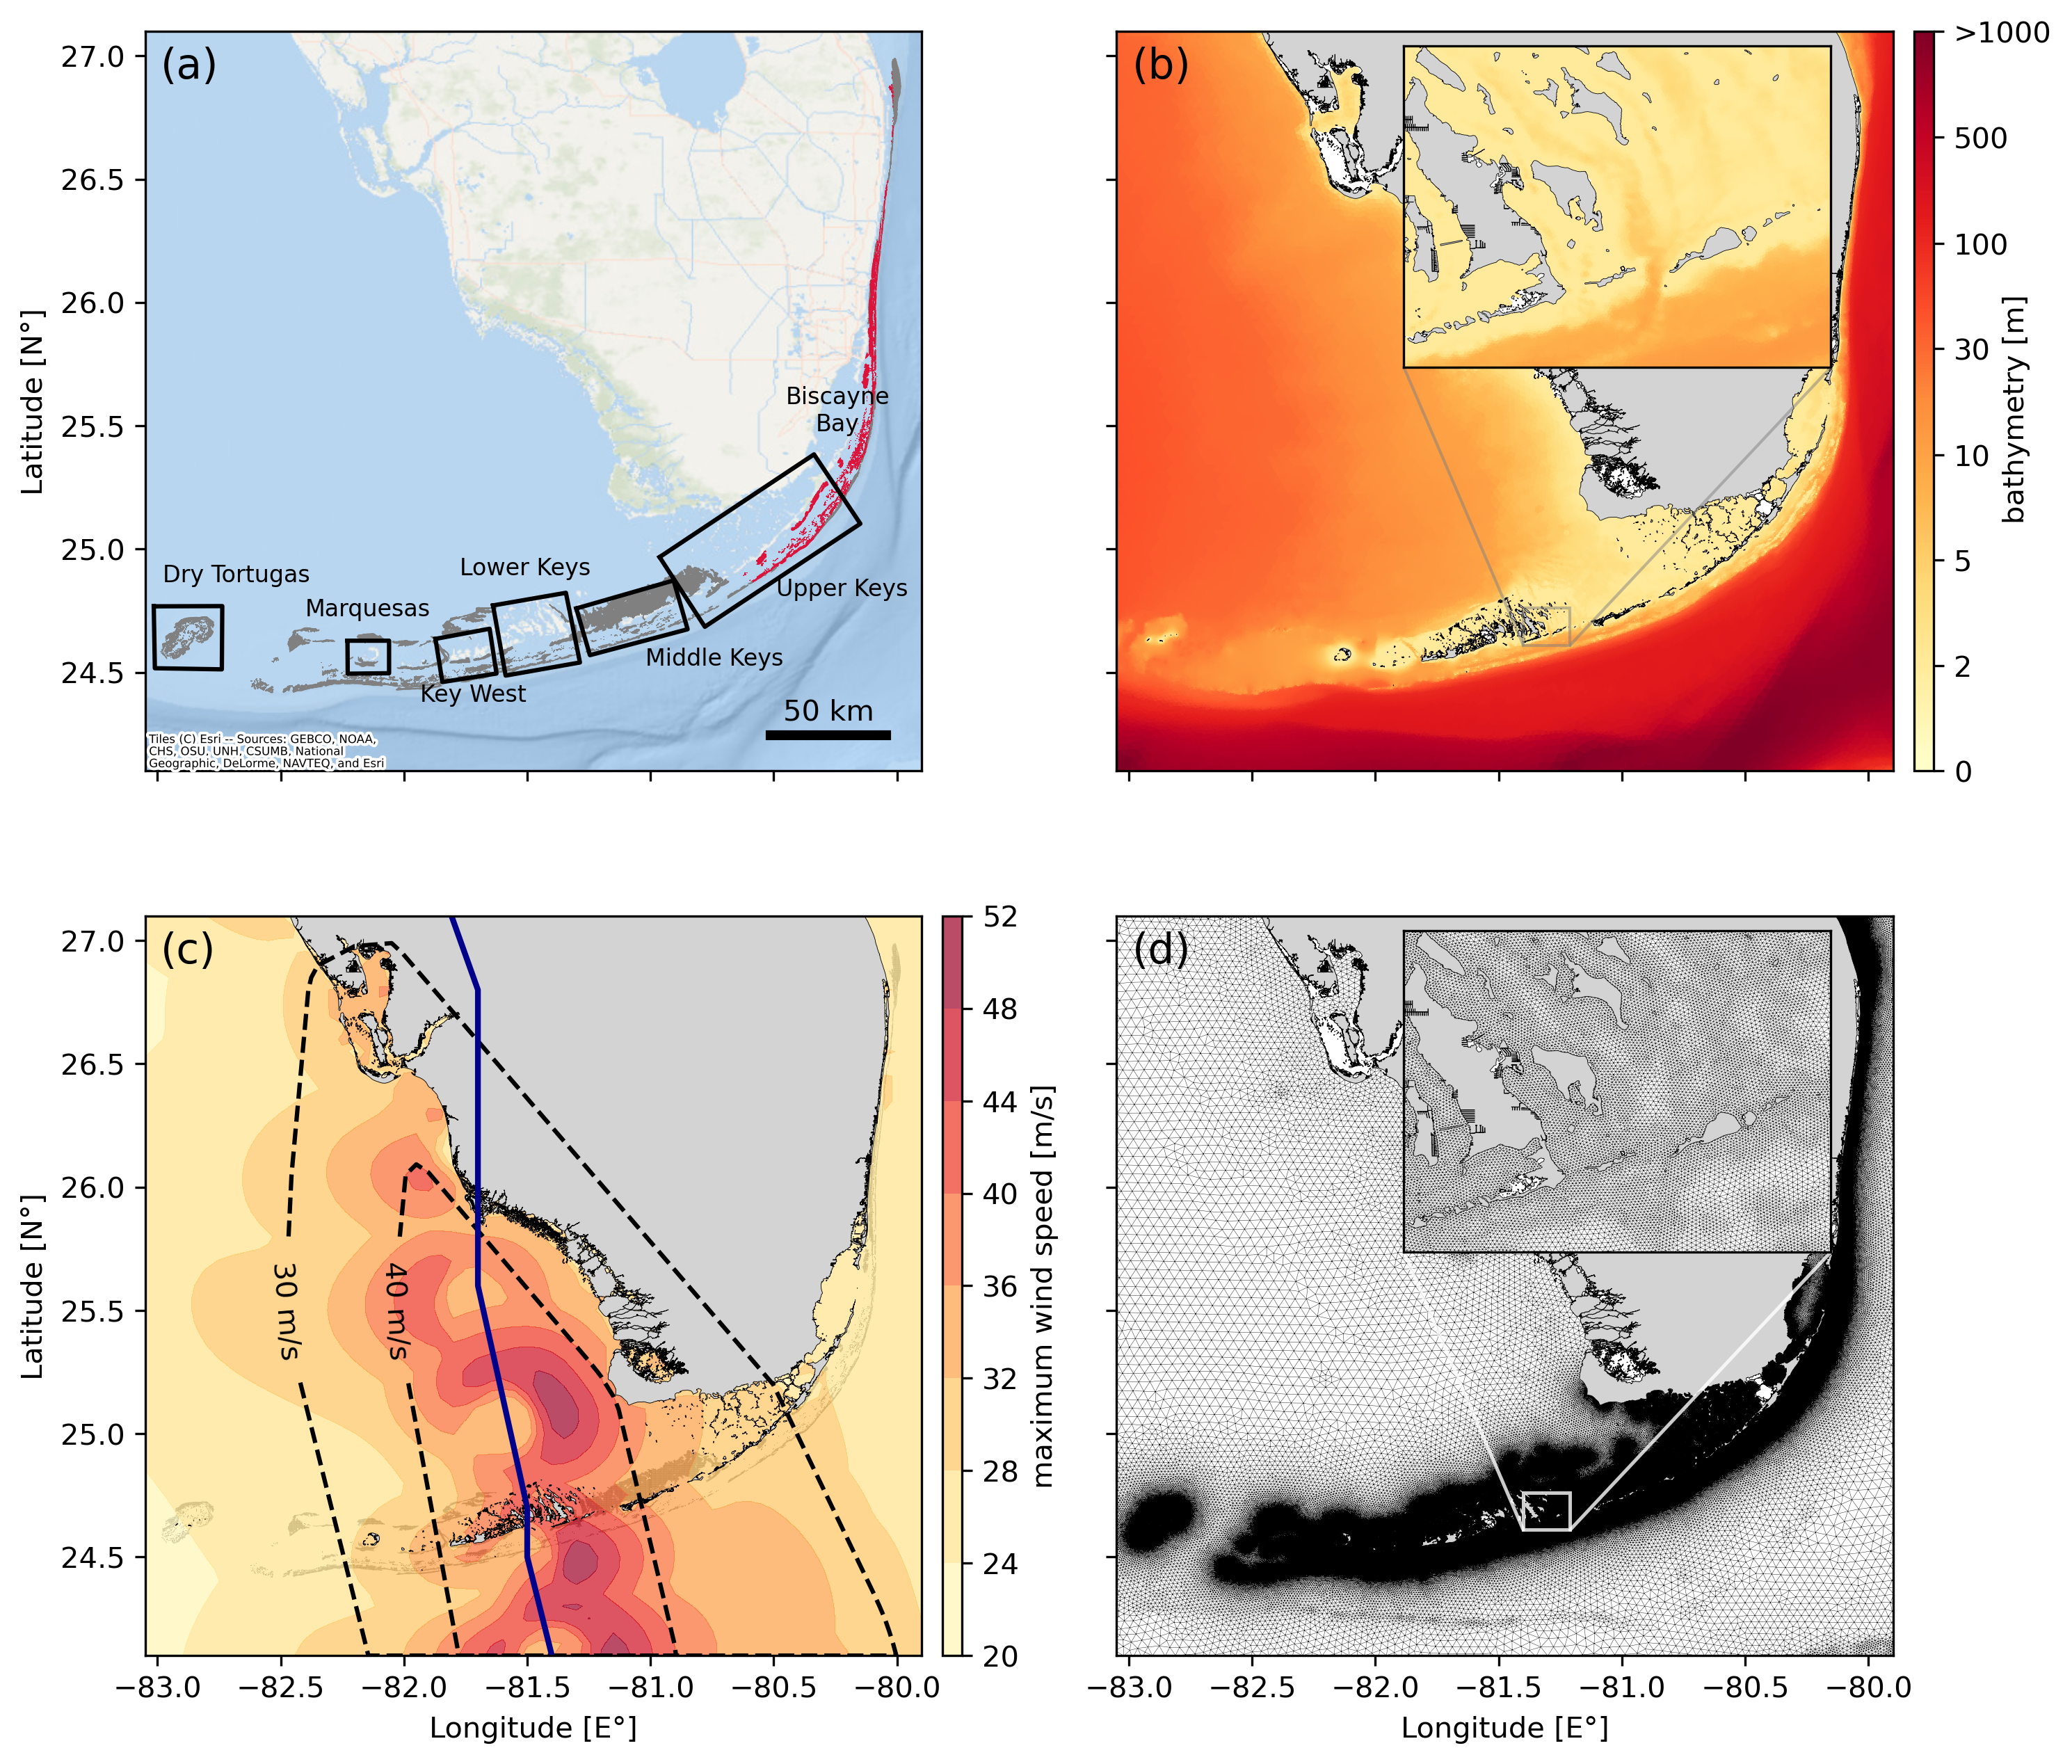
\includegraphics[width=.9\textwidth]{figures/fig_setup.png}
    \caption{Overview of the area of interest with \textbf{(a)} Florida's Coral Reef with healthy/susceptible reefs shown in dark grey and infected reefs shown in red, \textbf{(b)} the model bathymetry, \textbf{(c)} the maximum wind speed during Hurricane Irma (30 m/s and 40 m/s isolines in black dotted lines and track of Irma in dark blue) and (d) the model unstructured mesh whose resolution ranges from $\sim$100 m near the coast and reefs in FCR to $\sim$5 km offshore.}
    \label{fig:domain}
\end{figure}

\subsection{Coupled wave-current model}
We simulated ocean circulation during Irma using the high resolution coupled wave-current model SLIM+SWAN developed and validated during Hurricane Irma by \citep{DobbyIrma}. In this coupled model, ocean current are simulated using the 2D barotropic mode of the unstructured-grid multiscale ocean model SLIM, which solves the conservative form of the shallow water equations:
\begin{align}
\dfrac{\partial H}{\partial t} +\nabla\cdot(\UV) &= 0, \label{eq:slim_1}\\
\dfrac{\partial \UV}{\partial t}  + \nabla\cdot\left(\dfrac{\UV\UV}{H}\right) + f\mathbf{e}_z \times \UV &= gH\nabla(H-h) - \dfrac{1}{\rho}\nabla p_\text{atm} + \dfrac{1}{\rho}\text{\boldmath$\tau$}_s +\nabla\cdot(\nu\nabla\UV) - \dfrac{C_b}{H^2}|\UV|\UV + \gamma(\UV_\text{ref}-\UV), \label{eq:slim_2}
\end{align}
where $H$ is the water column height and $\UV$ is the depth-averaged transport; $f$ is the Coriolis coefficient; $g$ is the gravitational acceleration; $h$ is the bathymetry; $\nu$  is the Smagorinsky viscosity; $C_b$ is the bulk bottom drag coefficient; $p_\text{atm}$ is the atmospheric pressure; {\boldmath$\tau$}$_s = ${\boldmath$\tau$}$_s^\text{wind}$ + {\boldmath$\tau$}$_s^\text{waves}$ is the surface stress due to wind and waves. To withstand potential drying in parts of the model grid during the hurricane, these equations were solved using a wetting-drying algorithm \citep{Le2020Aug}. As most corals reefs are located at depth shallower than 20 m, 2D unstructured-grid models are able to accurately simulate the barotropic dynamics prevailing in shallow areas while allowing for a 100 m spatial resolution over reefs at a tractable computational cost. Furthermore, barotropic phenomena were indirectly captured by gradually relaxing the simulated transport towards a reference transport $\UV_\text{ref}$ with coefficient $\gamma$ in regions were water depth was exceeding $50$ m. This reference transport was obtained by depth integration of the velocity field produced by the operational model HYCOM \citep{Chassignet2007Mar}. This allowed the model to indirectly represent the mesoscale eddies occurring along the FC or south of FCR \citep{Frys2020}.

The wave component of the coupled model is the unstructured parallel version of the spectral wave model SWAN, which solves the action balance equation:
\begin{equation}
    \dfrac{\partial N}{\partial t} + \nabla_\mathbf{x}\cdot[(\mathbf{c}_g+\mathbf{u})N] + \dfrac{\partial }{\partial \theta}[c_\theta N] + \dfrac{\partial}{\partial \sigma}[c_\sigma N] = \dfrac{S_{in}+S_{ds}+S_{nl}}{\sigma}~, \label{eq:swan}
\end{equation}
where $N$ is the wave action density; $\theta$ is the wave propagation direction; $\sigma$ is the intrinsic wave frequency; $\mathbf{c}_g$ is the wave group velocity, $\mathbf{u}=\mathbf{U}/H$ is SLIM depth-averaged current velocity; $c_\theta$ and $c_\sigma$ are the propagation velocities in spectral space due to refraction and shifting in frequency due to variations in depth and currents; and $S_{in}$, $S_{ds}$, and $S_{nl}$ respectively represent wave growth by wind, wave decay and nonlinear transfers of wave energy through four and three-wave interactions, \ie~quadruplets and triplets. The wave and current components were coupled through the radiation stress gradient {\boldmath$\tau$}$_s^\text{waves}$, \ie~the force exerted by waves on currents, computed by SWAN and accounted for in Eq. \ref{eq:slim_2}. Moreover, the modeled wave energy spectra were used to compute the Stokes drift, \ie~the net drift in the direction of the wave propagation, as in \cite{DobbyIrma}. This wave-induced transport was used in combination with SLIM's depth-averaged current velocity to simulate the dispersal of coral larvae and disease agents.

The model bathymetry (Fig. \ref{fig:domain}b) was built by combining three data sources: the General Bathymetric Chart of the Ocean (GEBCO; 15 arc-seconds resolution), the Coastal Relief Model (NOAA National Geophysical Data Center, 2001; 3 arc-seconds resolution), and NOAA’s bathymetric Digital Elevation Model (National Centers for Environmental Information, 2018; 1/3 arc-seconds resolution). Hurricane Irma's wind field (Fig. \ref{fig:domain}c) was reconstructed using high-resolution H*Wind wind fields \citep{Powell1998Sep}. However, as H*Wind wind profiles did not cover the entirety of our domain, we combined it with a coarser wind field extracted from the European Centre for Medium-Range Weather Forecasts (ECMWF) ERA-5 dataset \citep{Hersbach2020Jul}. The pressure field during the passage of Irma was reproduced by merging ERA-5 data, for the baseline pressure field, with an idealized Holland pressure profile for the central depression \citep{DobbyIrma}. The tidal forcing data were recovered thanks to the OSU TOPEX/Poseidon Global Inverse Solution dataset \citep{Egbert2002Feb}. The coupled wave-current model equations were solved on an unstructured triangular mesh (Fig. \ref{fig:domain}d), whose resolution varies according to the bathymetry and distance to coast and to the reefs. It is composed of about $7 \times 10^5$ elements and its resolution ranges from approximately 100 m in FCR to 5 km offshore. The ocean circulation and wave models have been thoroughly validated on FCR with respect to ocean currents, sea surface elevation and significant wave height observations \citep{Frys2020, DobbyIrma, dobbelaere2022connecting}. Additional validation results for the currents during Sept. 2017 are provided in Appendix.

We simulated the ocean currents from August 1, 2017, to January 1, 2018, and wind-generated waves from September 5 to 15, 2017, to consider the hydrodynamic conditions prevailing before and after the passage of the hurricane. The simulated ocean currents and waves Stokes drift are combined to form a transport velocity that will drive the dispersal of coral larvae and disease agents (Fig. \ref{fig:currents}). In fair-weather conditions, the Stokes drift is usually negligible compared to the ocean currents. However, during a hurricane, it yields an extra velocity comparable to the ocean currents \citep{DobbyIrma} and it should hence be taken into account to simulate transport processes. One day before and after the passage of the hurricane, the combined ocean currents and Stokes drift show the usual flow patterns in FCR, which is dominated by the FC acting as a strong northeastward conveyor belt. The flow through the Lower Keys reef system and on the inner shelf is weak (Fig. \ref{fig:currents}a and d). In the hours preceding Irma's landfall in the Keys, the transport velocity becomes much more intense just offshore of the Lower Keys leading to a reversal of the transport dynamics westward with current speeds exceeding 1 m/s. The flow through the reef system is also much more intense (> 1m/s) and directed northward (Fig. \ref{fig:currents}b). After landfall, the transport velocity intensifies on the inner shelf and keeps on accelerating the flow through the Lower Keys. Offshore of the Keys, the flow starts to weaken and the eddy that led to the westward flow intensification moves west (Fig. \ref{fig:currents}d).

\begin{figure}
    \centering
    \includegraphics[width=.8\textwidth]{figures/fig_currents.png}
    \caption{Snapshots of the combined modeled depth-averaged currents and Stokes drift \textbf{(a)} 24h before landfall, \textbf{(b)} 3h before landfall, \textbf{(c)} 3h after landfall and (d) 24h after landfall. Note strong westward current developing offshore of the Lower Keys in panel (b). The trajectory of the hurricane is depicted by a solid blue line.}
    \label{fig:currents}
\end{figure}

\subsection{Transport model}
The simulated depth-averaged currents and Stokes drift were used to model the dispersal of both coral larvae and disease agents throughout FCR using a Lagrangian biophysical model. Coral spawning of several reef building species such as {\it Acropora cervicornis}, {\it Colpophyllia natans}, {\it Montastrea cavernosa}, {\it Orbicella faveolata} and {\it Pseudodiploria strigosa} usually takes place over two to three consecutive nights in about two to five days after the full moon of July and/or August (J. Figueiredo, pers. comm.). {\it M. cavernosa} (Mcav) can also spawn in September. According to the full moon of Sept. 2017, it was expected to spawn on the nights of Sept. 11-13. Given the proximity of the spawning of Mcav with the passage of Irma, we simulated the dispersal of larvae originating from two hypothetical spawning events, one occurring three nights before the passage of Irma (on Sept. 7-9) and one occurring three nights just after its passage (on Sept. 10-12).

The biophysical model represents larval mortality, acquisition and loss of competence, and settlement behaviours. For Mcav, it takes approximately 3.8 days for larvae to become competent after they have been spawned and hence acquire the ability to alter their buoyancy and settle on a reef. However, after a certain period, they exhaust their energy reserves, thereby losing this ability to settle on a reef. The competency acquisition and loss rates were set at 6.4\% and 1.6\% per day, respectively \citep{Kuba2016}. In addition, larvae may perish before reaching a reef to settle on. Larval mortality was modeled as a fixed daily probability of dying. It was set at a rate of 6.7\% per day, such that the average larval life expectancy was approximately 15 days \citep{Kuba2016}. When competent larvae are over a reef, we assume that can settle at a rate 20\% per hour \citep{king2023larval}.

Finally, once all the necessary parameters were set, virtual particles were released on all FCR reefs. The reef shapefile used to locate the different reefs in FCR was extracted from the “coral reefs and hardbottom” layer of the Unified Florida Reef Tract Map \citep{FWC2017Jan}. The polygons representing the reefs were then divided into 500 m $\times$ 500 m sub-reefs, amounting to 16,823 sub-reefs, in order to achieve results that were not dependent on reef size and to better represent the variability within one single reef as they can reach several kilometers. For each larval dispersal simulation, we seeded particles every 450 seconds from 15 min to 225 minutes after sunset and released in total 820 particles/km$^{2}$, which is much higher than the particle density threshold required to get connectivity results independent of the number of particles released \citep{Monroy2017Jan}. The dispersal simulations following both spawning events had a duration of three months. For the sake of simplicity and because of a lack of information, we assumed that all the reefs had the same Mcav coral cover, which is not the case in reality. However, as the purpose of this study is just to compare the connectivity with and without the hurricane, this assumption is acceptable.

For the disease agents, we considered a simulation starting on September 5 00:00 UTC and for which particles were released every 4 hours during 3 days with a density of 100 particles/km$^2$ ($\sim2.6\times 10^{6}$ particles in total). This allowed us to represent a situation where disease agents were already present in the water in the entire area where the disease was present before Irma. Disease agents were only released on reefs where the disease signs were observed prior to September 2017. The position of the disease front was estimated by \emphc{spatially interpolating the time of disease observation by kriging with a Gaussian semivariogramn using Python pyKrige module \citep{murphy2014pykrige}}, as in \cite{DobbySCTLD}. Disease observations were compiled from the 7 datasets used in \cite{muller2020spatial}: (i) Coral Reef Evaluation and Monitoring Project (CREMP; 2014–2017), (ii) CREMP Presence/Absence Data (CREMP P\_A; 2016–2017), (iii) Southeast Florida Coral Reef Evaluation and Monitoring Project (SECREMP; 2014–2017), (iv) Florida Reef Resilience Program Disturbance Response Monitoring (FRRP; 2014–2017), (v) Hurricane Irma Rapid Reef Assessment (IRMA; 2017, \cite{viehman2018}), (vi) the Southeast Florida Action Network citizen science program (SEAFAN; 2014–2017), and (vii) the Southefrn Coral Disease Margin field effort (2017 and 2018; \cite{neely2018surveying}). \emphc{However, as no case definition of the visual appearance and ecology of SCTLD was available before 2018 \citep{noaa2018}, these datasets compile observations of tissue loss consistent with SCTLD. Some disease observations might thus not correspond to SCTLD}. The other simulation started on September 12 00:00 UTC and also involved the release of particles during 3 days at the same rate. Disease agents were assumed to be transported within composite material (like dying tissue or resuspended sediments) mixed within the water column and hence driven by the barotropic currents. They were further assumed to have a half-life of 30 days \citep{DobbySCTLD}.


\subsection{Connectivity indicators}
The biophysical model simulations yield $16,823 \times 16,823$ connectivity matrices, denoted $C$ with entries $C_{ij}$. They represent the mass of particles released on sub-reef $i$ that settled on sub-reef $j$. It can be normalised by dividing each row by the number of particles released on the corresponding sub-reef to obtain the normalised connectivity matrix $\tilde{C}$. As such large matrices are very hard to analyse, we use instead graph theory tools to extract ecologically-meaningful connectivity indicators \citep{Thomas2014Jan,Frys2020,Figueiredo2022Jan}. We hence interpret the connectivity matrices as large directed graphs whose vertices represent reefs and edges correspond to non-zero entries in the matrix. The different connectivity indicators used in this study are defined in Table \ref{tab:indicators}. These are standard connectivity measures indicating the average dispersal distance or weighted connectivity length ($WCL$), the fraction of particles released that settles somewhere ($P^\text{settled}$), the potential to provide many particles to many reefs ($OC$) and the potential to receive many particles from many different reefs ($IC$).

\begin{table}
    \centering
    \begin{tabular}{p{0.25\textwidth}p{0.15\textwidth}p{0.5\textwidth}}
         \hline
         \textbf{Indicator} & \textbf{Formula} & \textbf{Description} \\
         \hline
         Weighted connectivity length  & $WCL_{i} = \dfrac{\sum_{j} \tilde{C}_{ij} L_{ij}}{\sum_{j} \tilde{C}_{ij}}$ & Average dispersal distance from origin to destination reef for all particles released over a reef  \\
         Proportion settled & $P^\text{settled}_{i} = \sum_{j} \tilde{C}_{ij}$ & Proportion of particles released by a reef that manage to settle \\
         Outgoing connectivity & $OC_{i} = N_{i}^{out} \sum_{j} \tilde{C}_{ij}$ & Number of outgoing connections originating from a given reef multiplied by the total mass of particles originating from this reef that settled on a reef \\
         Incoming connectivity & $IC_{i} = N_{i}^{in} \sum_{j} \tilde{C}_{ji}$ &  Number of incoming connections pointing to a given reef multiplied by the total mass of particles that settles on that reef\\
         \hline
    \end{tabular}
    \caption{Connectivity indicators used to analyze the dispersal of coral larvae and disease agents in the reef network.}
    \label{tab:indicators}
\end{table}

\subsection{Epidemiological model}
The connectivity matrices were then used to model disease propagation using the connectivity-based Susceptible-Infectious-Removed (SIR) epidemiological model developed by \citep{DobbySCTLD}. In this model, subpopulations of susceptible, infectious and removed corals are considered on each sub-reef polygon. Infection of susceptible corals on a given sub-reef polygon by infectious individuals from another sub-reef polygon is enabled when these reefs are connected in the disease networks and depends on the strength of the connection. Additionally, to account for coral resistance to the disease, infection within the same sub-reef polygon is only activated when the proportion of infectious corals on that sub-reef is greater than a given infection threshold $I_0$. Ref. \citep{DobbySCTLD} identified a well-defined range of infection threshold values for which the model accurately reproduced the observed spread of the disease between May 2018 and April 2019.

The disease connectivity matrices from both the hurricane and no-hurricane scenarios were input into the model, and simulations were conducted from September 1, 2017, to December 1, 2017, for various values of $I_0$ within the range of valid values identified in \citep{DobbySCTLD}. We employed the same calibrated transmission and removal parameters as in \citep{DobbySCTLD}, and the initial conditions of the model were calculated using a simplified SIR model following the methodology of \citep{DobbySCTLD}. Furthermore, the rows and columns corresponding to the so-called '\textit{Vaca Reef}' (Fig. \ref{fig:propagation}, \citealp{Frys2020}), which is particularly large but with a very low coral cover, were removed from the connectivity matrices to avoid an overestimation of the disease propagation \cite{DobbySCTLD}. For each simulation, the total infected area and the distance traveled by the disease front were computed.

% =============== %
% === RESULTS === %
% =============== %
\section{Results}
Hurricane Irma's impact on larval and disease connectivity has been assessed by comparing dispersal patterns initiated before and after the passage of the hurricane on Sept. 10 at 9am EDT (1pm UTC). For coral larvae, we considered two hypothetical spawning events of {\it Montastrea cavernosa} (Mcav) occurring on Sept. 7-9 and on Sept. 10-12. For the disease, we considered disease agents produced on Sept. 5-7 and on Sept. 12-14. Releasing disease agents earlier allowed us to better represent the situation prevailing during the passage of the hurricane where disease agents were already present in the water in the entire area affected by the disease. All the graphs presented in this section display relative changes computed by comparing larval and disease dispersal simulations impacted by the passage of the hurricane to similar simulations initiated just after its passage. For each connectivity indicator, we present both its relative change spatial distribution and its frequency density histogram. Since the latter is generally not normally distributed, the description of the results focuses on the median rather than on the mean of the distributions.

% Larval dispersal
% ----------------
\subsection{Larval dispersal}
The relative changes to the four connectivity indicators clearly highlight a difference between the western and eastern parts of the hurricane's track (Fig. \ref{fig:Larvae}). While the passage of Irma led to a global increase of the WCL with a median relative change of 18\%, this increase is most apparent for the reefs west of the track (Fig. \ref{fig:Larvae}a). Almost all these reefs saw their WCL substantially increase, with more than ten-fold increases observed for certain reefs, such as those in the Dry Tortugas and south of the Marquesas. Conversely, east of the hurricane track, the variability was more pronounced with alternating patches of WCL increase and decrease present on both the inner and outer shelves.

\begin{figure}[tbp]
    \centering
    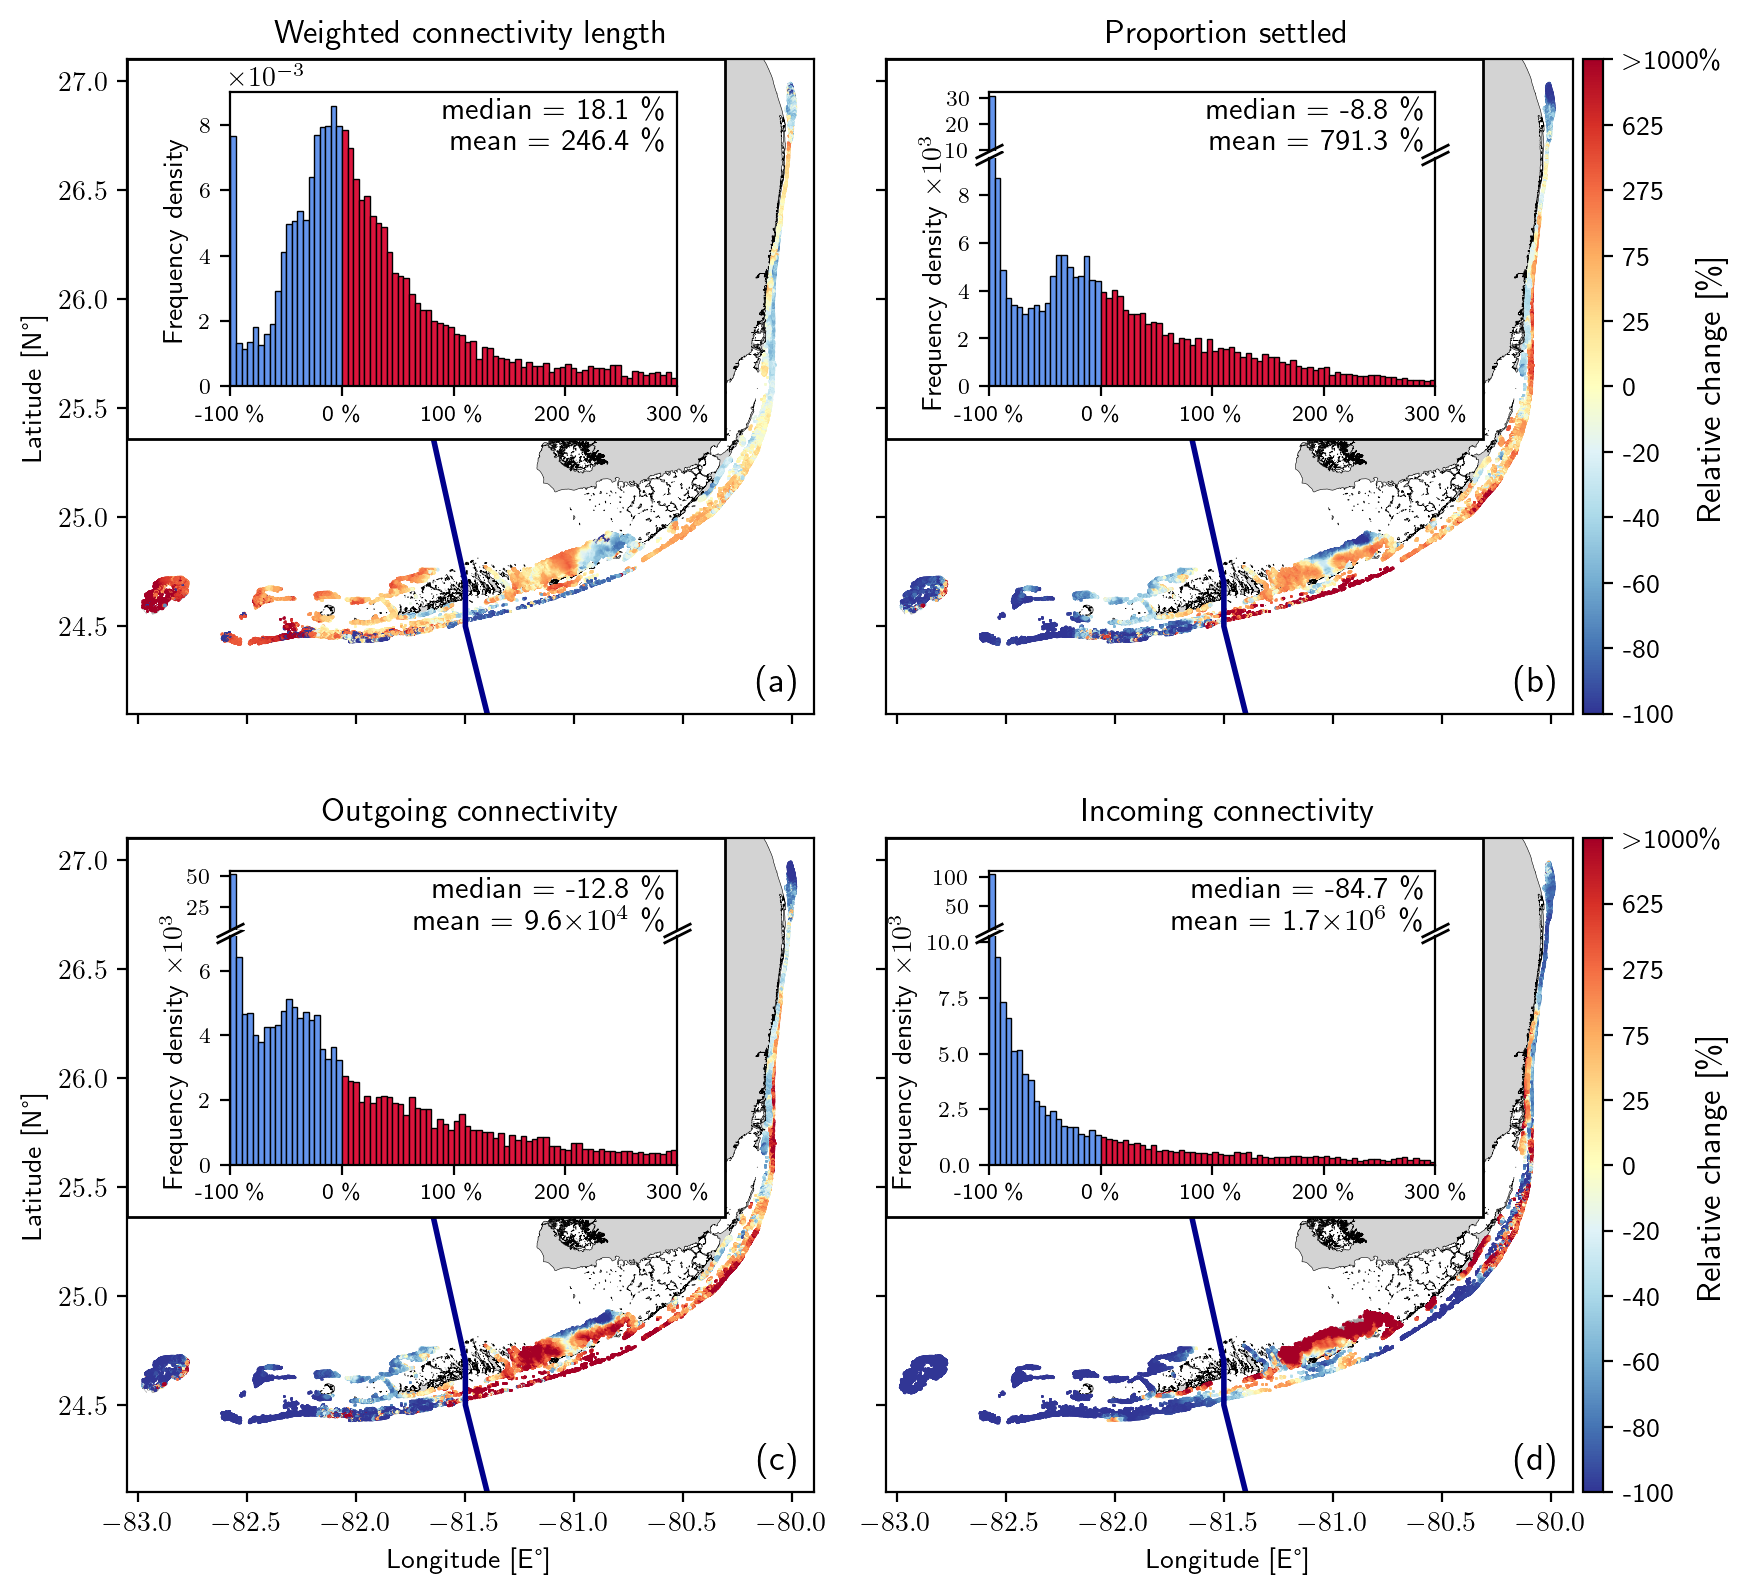
\includegraphics[width=0.9\textwidth]{figures/fig_connex_coral.png}
    \caption{Spatial distributions alongside frequency density histograms illustrating the relative changes induced by Hurricane Irma in larval \textbf{(a)} weighted connectivity length, \textbf{(b)} proportion settled, \textbf{(c)} outgoing connectivity, and \textbf{(d)} incoming connectivity. The trajectory of Hurricane Irma is depicted by a solid blue line. The horizontal axis of the histograms has been cropped to 300\% to improve readability.}
    \label{fig:Larvae}
\end{figure}

Model results also show that Irma strongly impacted the proportion of larvae that settles (Fig. \ref{fig:Larvae}b). While the median of this change is slightly negative (-8.8\%), the spatial distribution shows large variations. Reefs situated west of the track predominantly experienced a strong decrease in the proportion of their larvae that settled, suggesting that larvae are transported to areas lacking coral reefs or that their mortality increased as they take longer to settle. In contrast, the offshore reefs located east of the track witnessed a substantial increase in their proportion settled, sometimes exceeding ten-fold. West of the hurricane track and on the Middle Key's outer shelf, WCL and proportion settled are inversely correlated as reefs that observed an increase in their WCL generally also witnessed a decrease in their proportion settled and vice versa. This correlation however does not hold further north in the track.

%\dobby{\centering\begin{tabular}{l|cccc}
%        &  WCL   & propSet   &  outCon   &   inCon \\
%\hline
%WCL  &  1.000000 & -0.024694 & -0.012497 & -0.009475 \\
%propSet & -0.024694 &  1.000000 &  0.888036 & -0.002763 \\
%outCon  & -0.012497 &  0.888036 &  1.000000 & -0.001338 \\
%inCon   & -0.009475 & -0.002763 & -0.001338 &  1.000000 \\
%\end{tabular}}

The simulated change in outgoing connectivity exhibits a similar pattern as the change in the proportion settled (Fig. \ref{fig:Larvae}c). Overall, the median is again negative (-12.8\%) but the differences between the reefs are even more striking. A majority of the reefs west of the track witnessed a significant reduction in their source index, particularly for reefs in the Dry Tortugas, near the Marquesas, and on the outer shelf. These are the same reefs for which the increase in WCL was the largest, as was already evident in the proportion settled distribution. East of the track, there are reefs with considerable increases, especially in the Middle Keys and on the outer shelf.

Lastly, the relative change in incoming connectivity underscores that only a few reefs strongly benefited from the shifts in connectivity patterns driven by Irma (Fig. \ref{fig:Larvae}d). The relative change distribution's median is notably low (-84.7\%), indicating that the vast majority of reefs witnessed a decline in their larval supply. Most reefs west of the track and those east of the track on the outer shelf experienced a pronounced decrease, often resulting in a complete disappearance of larval supply. The clear beneficiaries were the inner-shelf reefs in the Middle Keys, reefs in the Upper Keys, and some reefs near the coast north of Biscayne Bay.

% Disease dispersal
% -----------------
\subsection{Disease dispersal}
As our objective was to determine whether Irma accelerated the spread of SCTLD, we focused only on connections from reefs that were infected at the time of Irma's passage (refer to the distribution in Fig. \ref{fig:domain}a) to those that were healthy (\ie, susceptible) within the connectivity matrix. Consequently, metrics such as WCL, proportion settled, and outgoing connectivity were calculated only for infected reefs, while incoming connectivity was calculated only for susceptible reefs.

\begin{figure}[tbp]
    \centering
    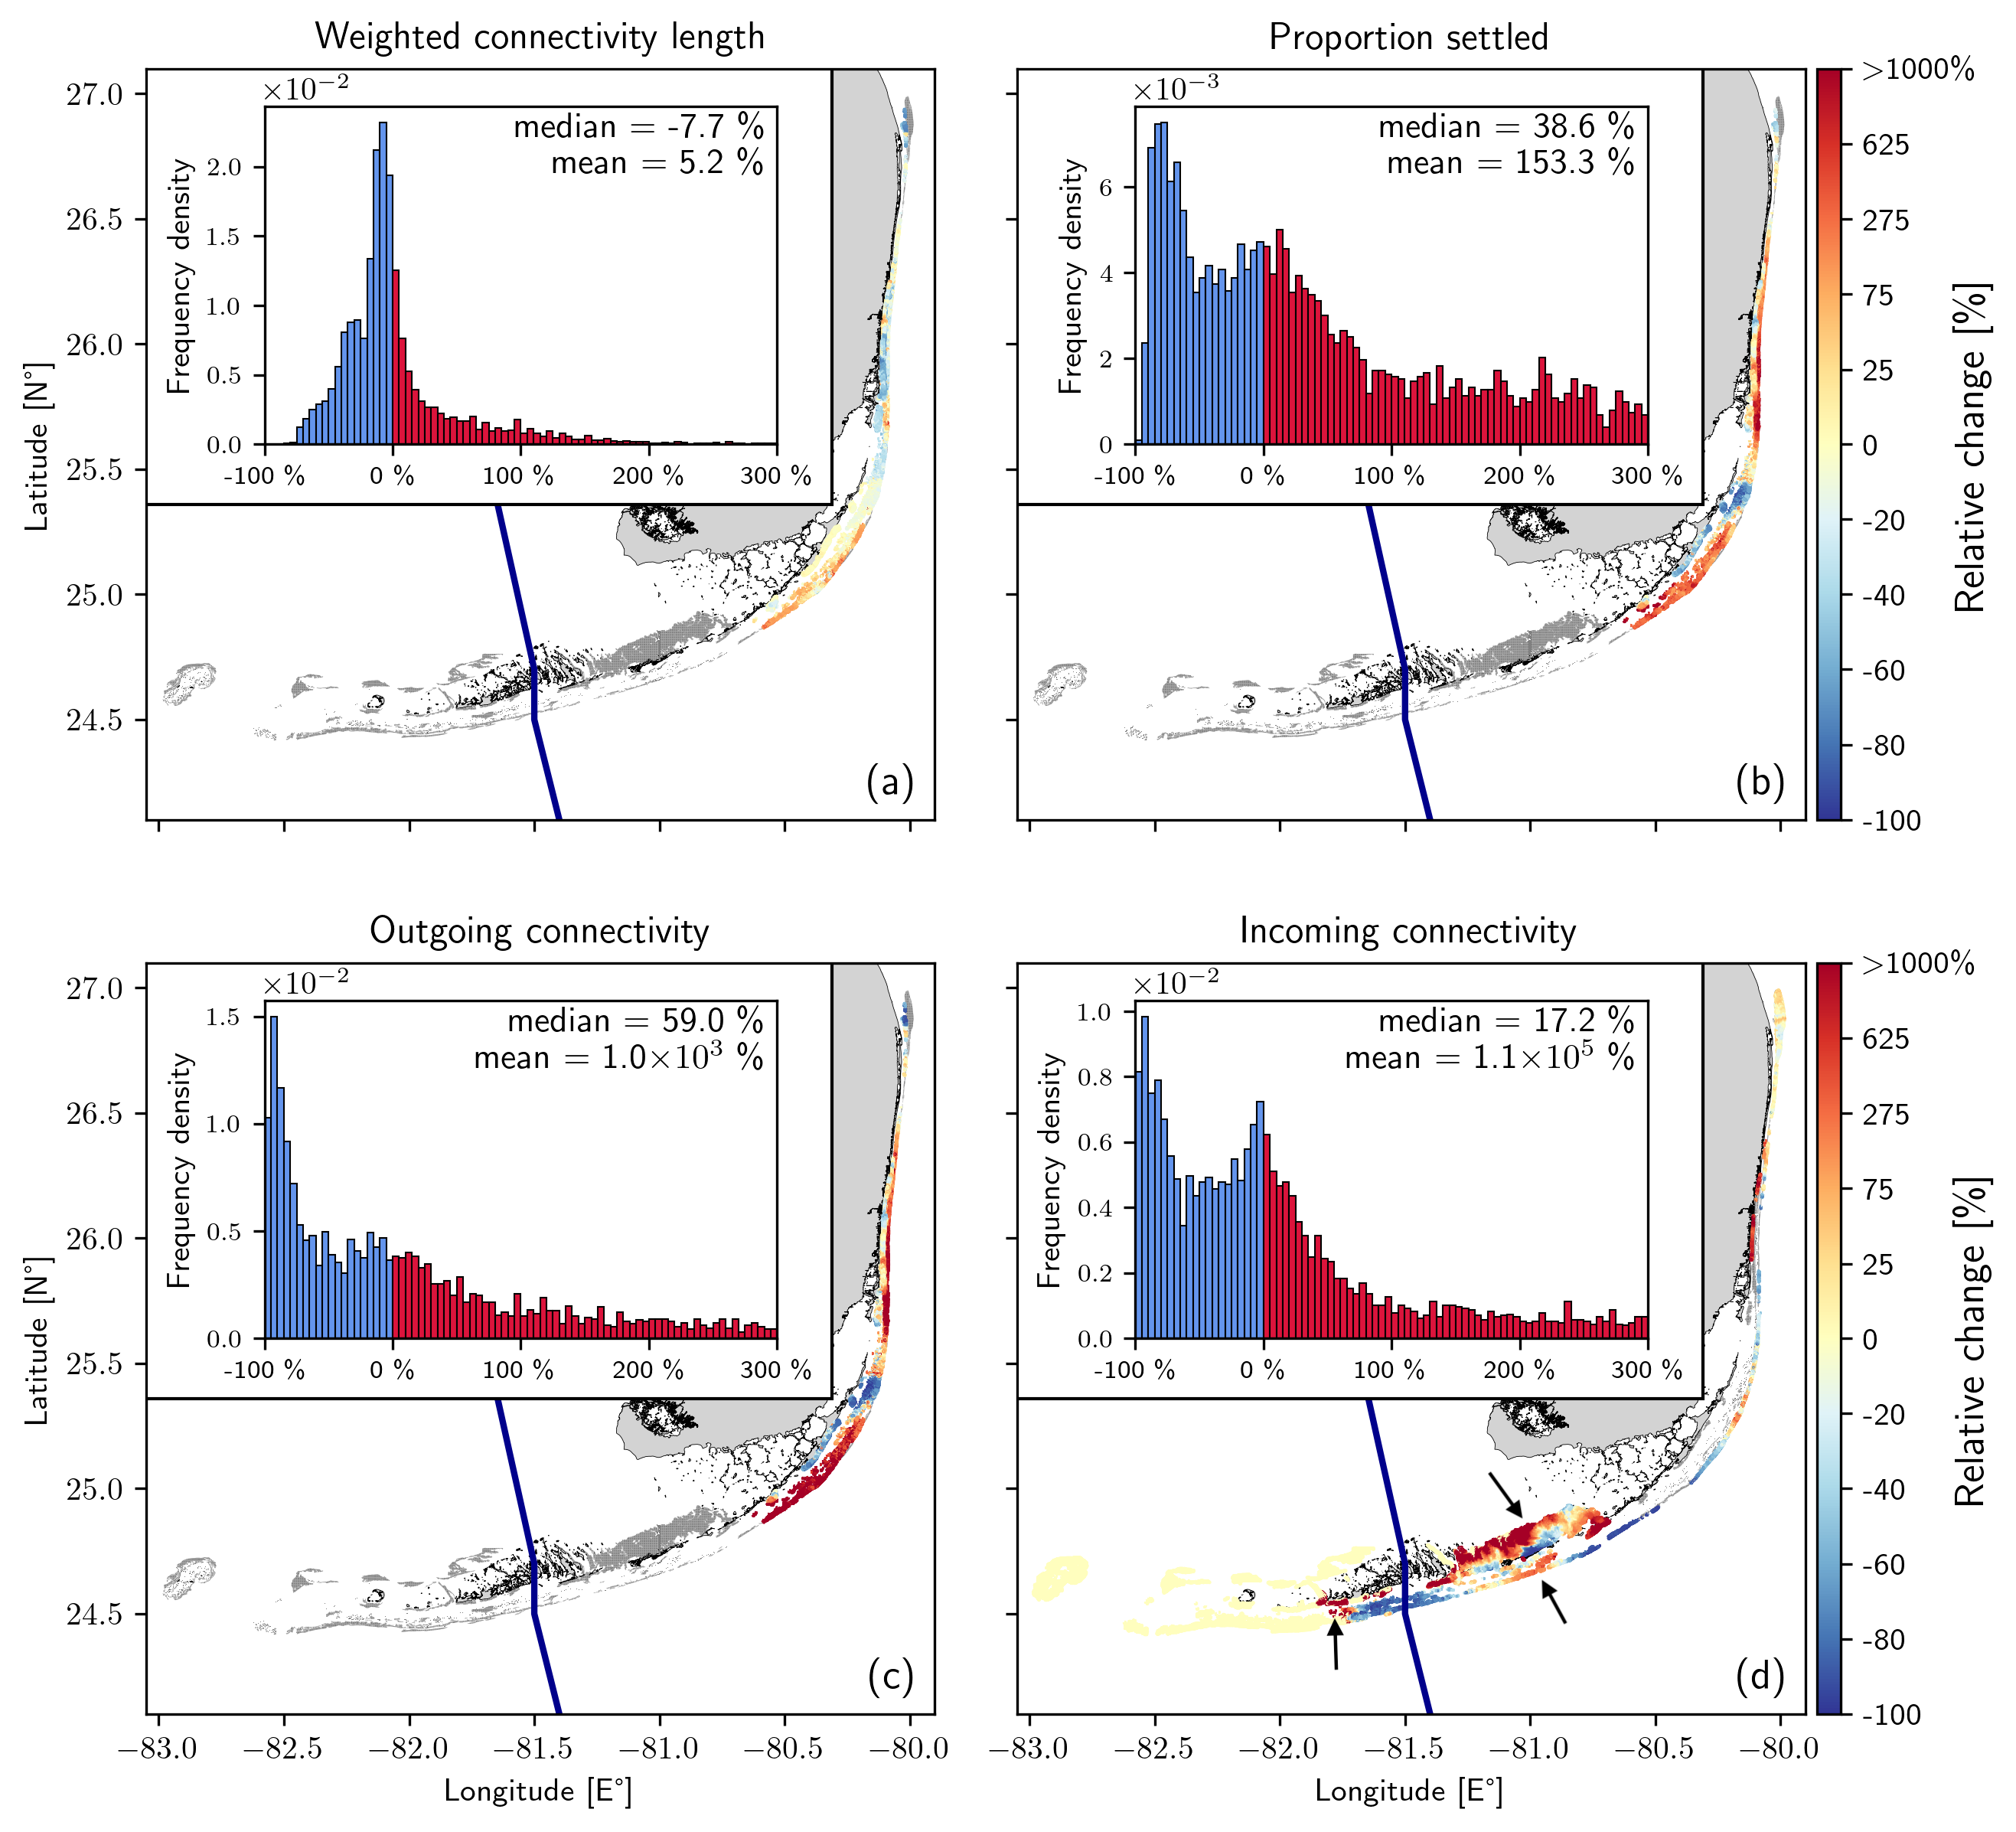
\includegraphics[width=0.9\textwidth]{figures/fig_connex_sctld_b.png}
    \caption{Same as Fig. \ref{fig:Larvae} for disease dispersal. Note that the zero values in panel (d) west of the Lower Keys correspond to reefs for which there is no incoming connectivity both with and without Irma. The relative change is thus undefined and they are not considered in the frequency density histogram. Arrows in panel (d) highlight patches of susceptible reefs that experienced a surge in incoming disease connectivity following the passage of Irma. }
    \label{fig:SCTLD}
\end{figure}

Although the distribution of relative changes in WCL indicates that the majority of infected reefs saw a reduction in the distance over which they could transmit disease agents during the hurricane's passage, some reefs experienced a strong increase in WCL (Fig. \ref{fig:SCTLD}a). This surge was primarily due to infected reefs in the Upper Keys, which were at the forefront of the SCTLD epidemic in September 2017. Some of these reefs witnessed their WCL more than double in the aftermath of Irma's passage. Conversely, infected reefs further north generally experienced a decrease in their WCL.

Examining the proportion of disease agents that successfully reached a susceptible reef, we notice a pronounced increase in the median of the relative change histogram, suggesting a global increase for the majority of reefs (Fig. \ref{fig:SCTLD}b). Infected reefs situated at the frontline of the epidemic, which experienced an increase in their WCL, also witnessed a significant increase in the proportion of disease agents they produce that reached susceptible reefs. Similarly, infected reefs further north, where the WCL decreased, also saw a comparable increase in their proportion settled.

The distribution of the simulated outgoing connectivity indicator reinforces the previous findings (Fig. \ref{fig:SCTLD}c). It highlights a cluster of infected reefs in the Upper Keys, at the forefront of the epidemic, that underwent a substantial increase in their outgoing connectivity index, often exceeding tenfold. This implies that these infected reefs transmitted more disease agents to a greater number of susceptible reefs due to the passage of the hurricane. On the whole, the median of the frequency density distribution saw a significant increase (+59\%), suggesting that the majority of infected reefs became more potent sources of disease, thereby accelerating the progression of the epidemic.

The distribution of incoming connectivity pinpoints which susceptible reefs could have received the most disease agents from the infected reefs (Fig. \ref{fig:SCTLD}d). Three areas stand out: a large reef cluster on the inner shelf of the Middle Keys, almost contiguous to the disease front, a smaller cluster of reefs on the outer shelf of the Middle Keys, and an even smaller cluster on the outer shelf of the Lower Keys (see arrows in Fig. \ref{fig:SCTLD}d). The first and last of these areas correspond to substantial increases in incoming disease agents, often exceeding tenfold. This suggests that Irma facilitated the disease's spread to reefs far from the disease front and into areas like the inner shelf, which would typically be more challenging for disease agents to reach under normal flow conditions. Overall, it appears that the majority of susceptible reefs experienced an increase in their exposure to disease agents, with a relative change median of +17.2\%.

Finally, we ran epidemiological model simulations with the disease connectivity matrices obtained with and without the hurricane. Model results suggest that the passage of Irma helped the disease to
propagate further away and affect more reefs (Fig. \ref{fig:propagation}). It drove the disease agents both shoreward and further westward, causing the disease to spread to reefs near Lower Matecumbe Key instead of reefs directly adjacent to the initial disease front. On average, this "leapfrog" caused a 28.9\% increase in propagation distance and an 87.0\% in affected area compared to the reference simulation. Dividing the difference in disease propagation between the hurricane and reference (\ie not influenced by Irma) simulations by the disease propagation speed of the reference simulation, we obtain that the impact of the hurricane was equivalent to about 25 days of disease spread under fair weather condition.

The results of our epidemiological model were validated against disease observations made after the passage of the hurricane (see red triangles in Fig. \ref{fig:propagation}). By mid-October, SCTLD lesions were observed at 3 sites ahead of the disease front location before the hurricane. One of these disease observations is rather close to the initial front position and on a reef that was not predicted to be infected when taking Irma into account. However, the two other sites correspond to reefs at the forefront of the area that we identified as potentially infected by long-distance disease agents dispersal driven by the hurricane. Those sites are located quite faraway from the initial disease front, which supports the idea that the passage of Irma accelerated the spread of the SCTLD epidemic.

\emphc{Thomas: Check the text above is OK and maybe say something about disease observations until Dec. 1 2017. Were there no observations at all or just no new lesions observations?}

\begin{figure}[tbp]
    \centering
    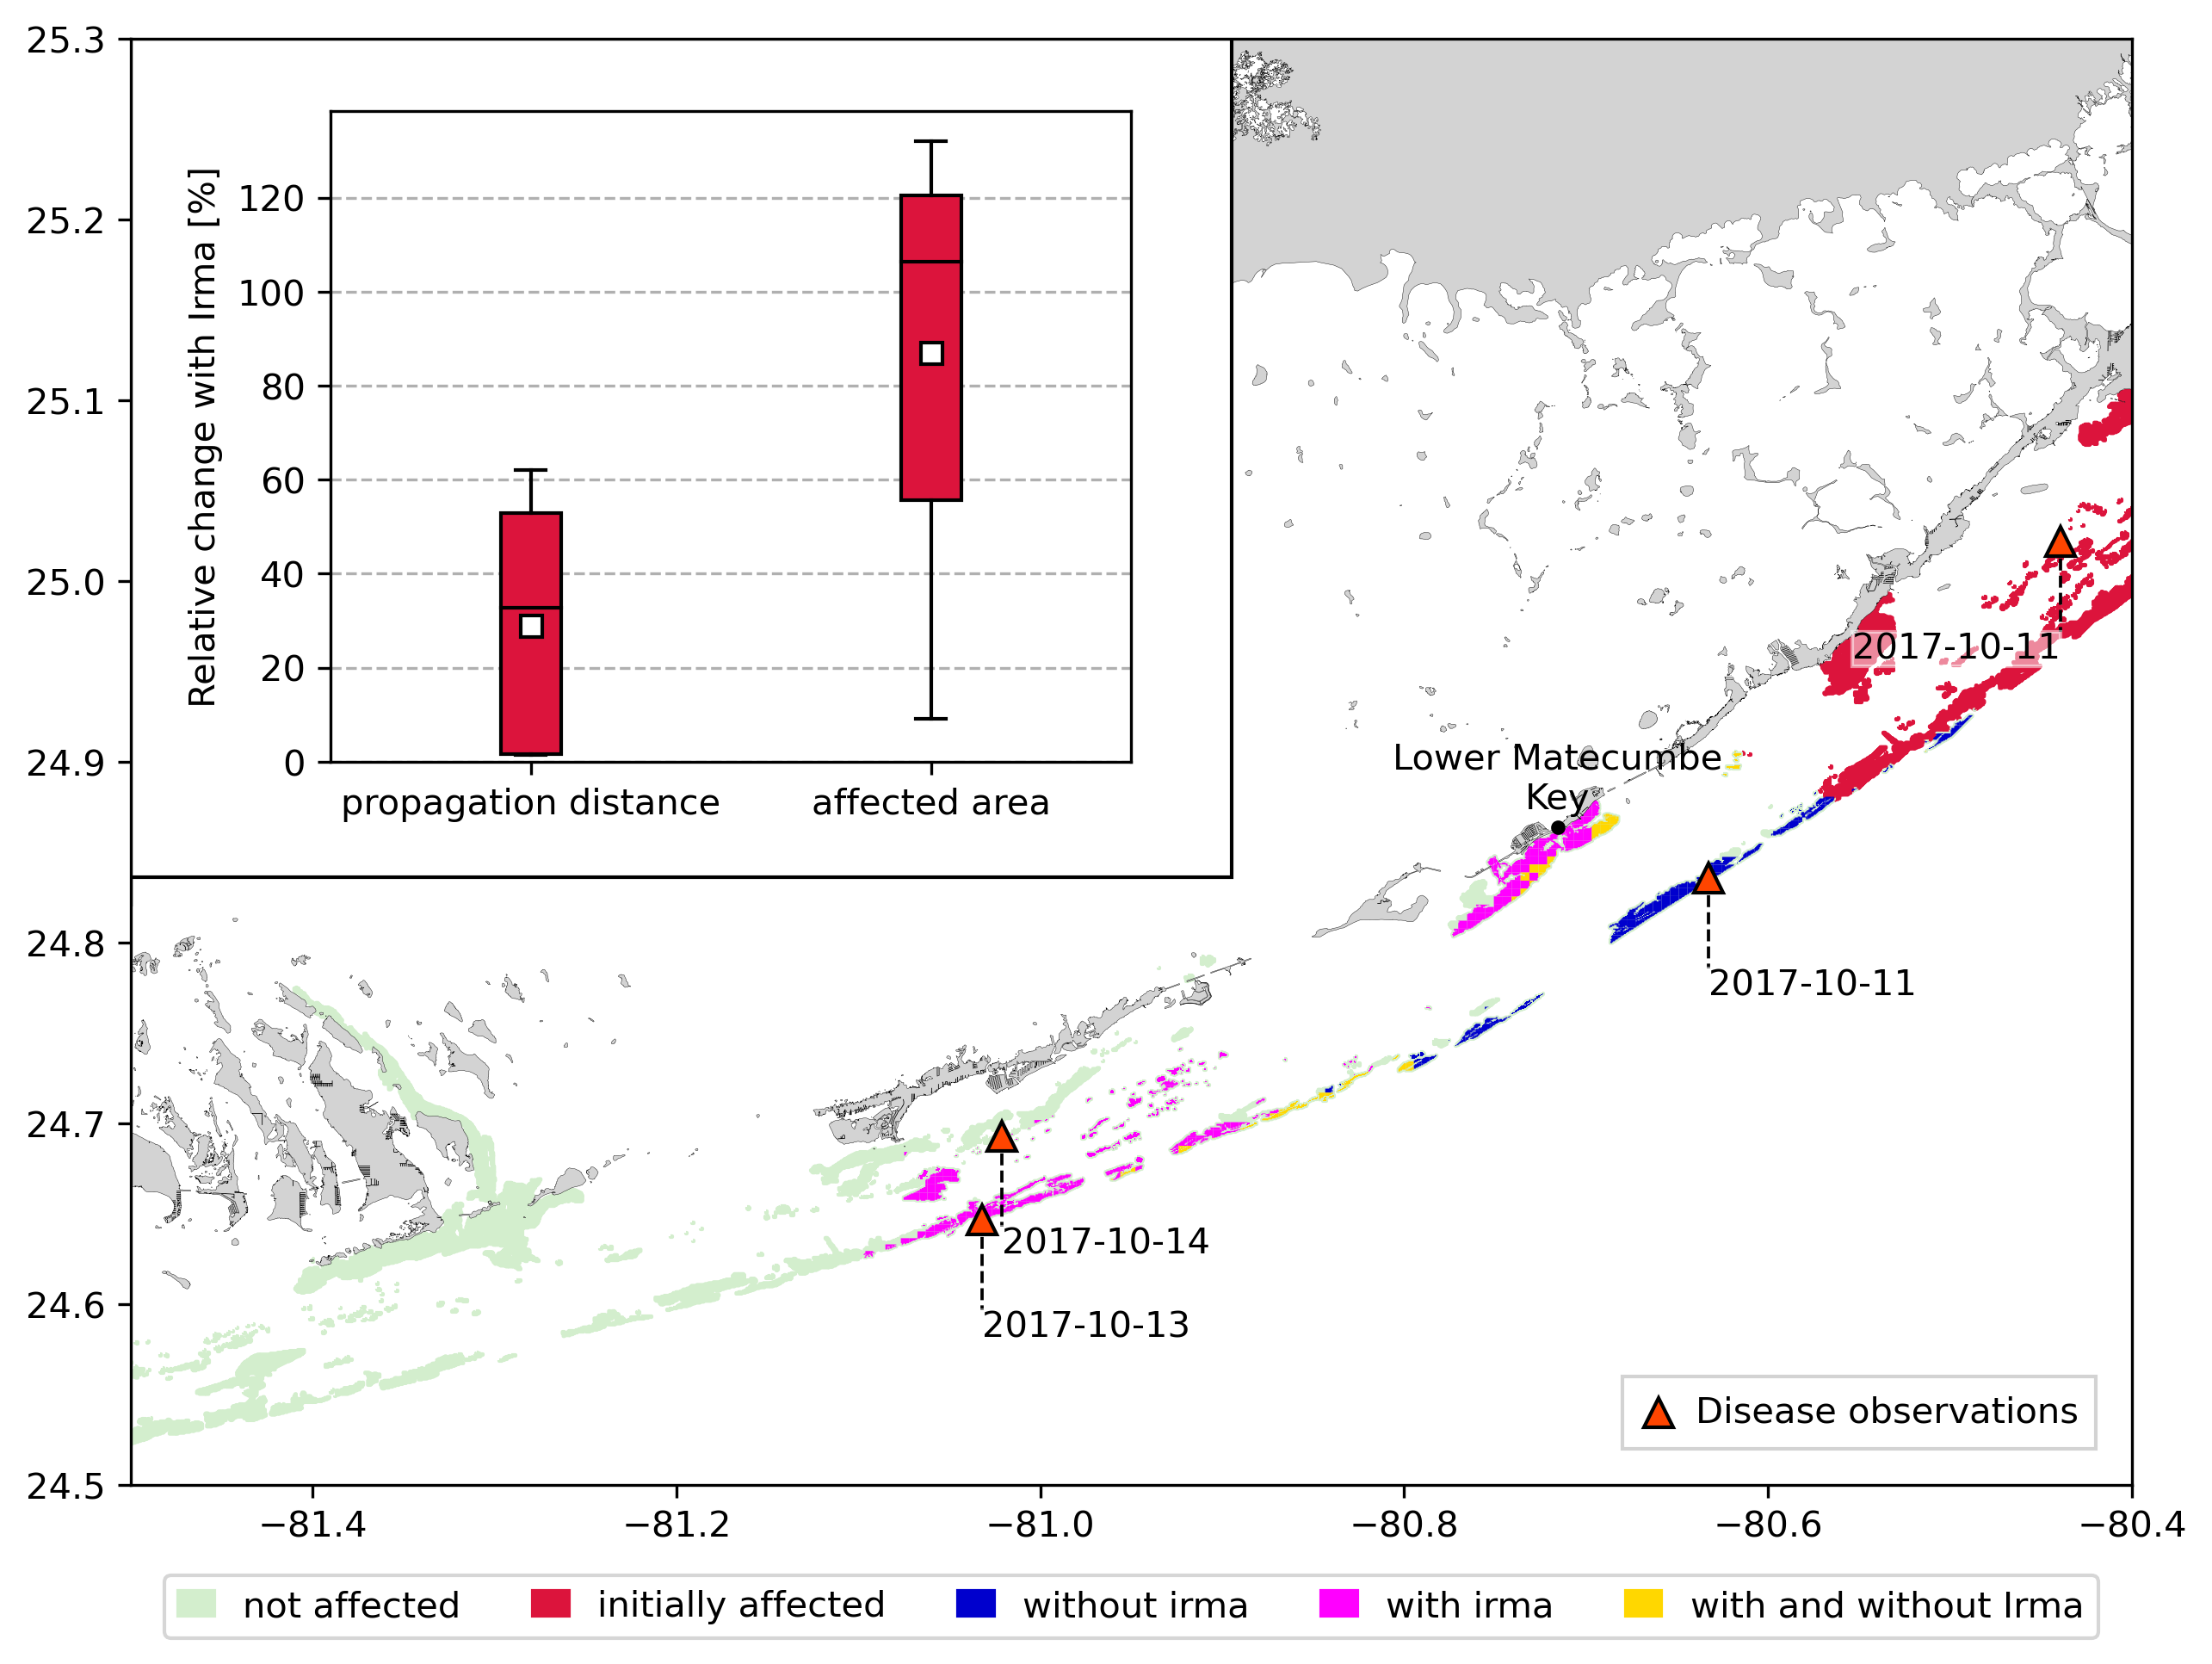
\includegraphics[width=.8\textwidth]{figures/propagation_boxplot_obs.png}
    \caption{
        Propagatthe disease simulated by the connectivity-based epidemiological model between Sept. 1 and Dec. 1 2017 using the reference (purple) and hurricane (orange) connectivity matrices. Reefs affected by SCTLD prior to Sep 1 2017 are shown in red and fully susceptible reefs in green. Disease observations until Dec. 1 2017 are shown with red triangles. The upper left graph shows the relative change in the distance travelled by the disease front and the total affected area when accounting for Irma different values of the model's infection threshold. The central lines of the boxes and the white square respectively indicate the median and mean of the relative change, the bottom and bottom of the boxes indicate the 25th and 75th percentiles respectively, while the minimum and maximum of the relative change are indicated by the bottom and top whiskers. On average, the hurricane caused  a 28.9\% increase in disease propagation distance and an 87.0\% increase in affected area, equivalent to about 25 days of disease propagation under fair weather conditions.
    }\label{fig:propagation}
\end{figure}

% ================================== %
% === DISCUSSION AND CONCLUSIONS === %
% ================================== %
\section{Discussion and conclusions}

% § to summarize main messages
By taking Hurricane Irma as a test case, our study illustrates how major hurricanes' impact on connectivity can be a double-edged sword; they promote genetic mixing among coral reefs, can foster the recolonization of remote areas and facilitate range expansion but they can also accelerate the spread of coral diseases and other threats to coral reefs. The main consequences of a hurricane on the hydrodynamics are wind-wave-current interactions that intensify and deflect the usual transport pathways. As a result, both coral larvae and coral disease agents can be transported further away and reach reefs they would not normally reach. In the case of the SCTLD epidemic, which had already covered about half of FCR at the time of Irma's passage, it was able to advance over a distance that would typically take about a month to be covered under fair weather conditions. However, at the same time, larval exchanges between separated coral reefs became longer, with half of all reefs experiencing an increase of more than 18\%. This means that genes carrying some advantageous features were able to spread more rapidly through the coral reef ecosystem, hence bolstering its resilience and adaptation.

% § on more general conclusions (left vs right side of track)
More generally, our study illustrates the varying impacts a hurricane can have on connectivity on either side of its track. In the Northern Hemisphere, hurricanes rotate counterclockwise. Consequently, for a hurricane approaching perpendicular to the shore, the wind-driven flow will be directed towards the coast on the right side of the track and towards the sea on the left side. There will further be a wave-driven flow acceleration along the shore in the area where the hurricane track intersects the shoreline, which can reverse the direction of the main transport pathways. For barrier reefs like Florida's Coral Reef or the Mesoamerican Reef, this results in shorter and stronger larval exchanges on the right side of the track. Conversely, on the left side, there will be longer and weaker exchanges. In the Southern Hemisphere, hurricanes rotate clockwise and the opposite conclusions hold. While these general patterns are influenced by the specific topography of the reef system, they nonetheless suggest that reefs on the right side of the track (where hurricane winds are stronger) may benefit more from changes in larval connectivity patterns.

% § on coral connectivity
Despite its fleeting occurrence, Hurricane Irma strongly influenced larval transport pathways. In our hypothetical test case comparing two spawning events, one before and the other after the passage of the hurricane, it resulted in a more intense flushing of the larvae away from their source reef. In the Lower Keys, Irma drove larvae offshore, where currents are stronger, and hence increased the distance they could be transported over while diminishing the proportion of larvae that eventually settled and the outgoing connectivity index. In that area, Irma promoted longer but also weaker connections, thereby allowing longer-distance genetic mixing within FCR. From the Middle Keys and further north, Irma drove larvae inshore hence promoting exchanges from outer-shelf to inner-shelf reefs in the Middle Keys, hence potentially fostering the recolonization of inner shelf reefs, which currently have a very low coral cover.

The overall decrease in incoming connectivity indicates that only a minority of reefs benefited from the alterations of larval dispersal pathways. In our test case, three regions - the inner-shelf Middle Keys, the Upper Keys, and reefs north of Biscayne Bay - experienced the greatest enhancement of larval supply due to the hurricane, albeit at the expense of other areas. These regions likely enhanced their resilience and genetic diversity by receiving larvae from more distant reefs, while the majority of FCR experienced a decrease in incoming connectivity. This outcome is not surprising as the current distribution of coral reefs mirrors long-term connectivity patterns. Reefs tend to thrive in areas with a robust larval supply. Therefore, significant alterations to these established connectivity patterns would likely result in a reduction in larval supply for most reefs. Such changes could however be sufficient to bolster both genetic exchanges and the colonization of new areas.

% § on disease dispersal
All disease connectivity indicators point towards Hurricane Irma acting as a superspreader event for SCTLD, thereby accelerating the epidemic's spread. Indeed, while the hurricane-induced shoreward flow in the northern part of FCR shortened the dispersal of disease agents, the reefs at the frontline of the SCTLD epidemic witnessed a combined increase of WCL, outgoing connectivity index, and proportion settled. Consequently, Irma facilitated the successful settlement of the disease onto a larger number of susceptible reefs and aided the disease's propagation over greater distances, particularly for pathogens originating from reefs at the epidemic's frontline. This result was further demonstrated by epidemiological simulations suggesting that the impact of Irma was equivalent to about 25 days of disease propagation under fair weather conditions. This accelerated spread was due to the disease propagating through the reefs with an increased incoming connectivity under the effect of Irma. The location of the disease front on the right of the hurricane's track favoured this enhanced transport as it allowed disease agents to be carried away by the strong westward alongshore current that developed offshore of the landfall location (Fig. \ref{fig:currents}b). This hurricane's effect on disease agents dispersal would also apply to other waterborne threats to coral reefs such as pollutants, sediment plumes and predatory species larvae such as crown-of-thorn starfishes \citep{pratchett2017thirty}. The latter are however not present in Florida.

Our findings are consistent with previous studies that have shown that hurricanes are a vector of species range expansion, particularly in the Caribbean and Gulf of Mexico, which are frequently impacted by hurricanes. For instance, Ref. \cite{Johnston2015hurricanes} have linked the expansion patterns of the invasive lionfish from Florida to the Bahamas to hurricane frequency. They showed that hurricanes could have sufficiently disturbed the Florida Current to allow lionfish larvae to be transported across the Florida Straits and reach the Bahamas, where they rapidly spread through the archipelago. Similarly, Ref. \cite{kennedy2020hurricanes} showed that hurricanes, and particularly Hurricane Irma, fostered Florida mangrove pole-ward range expansion by opening short windows of long-distance dispersal and hence accelerated the species range shift.  Multiple marine species with dispersal-driven reproduction occurring within the hurricane season can therefore take advantage of these extreme weather events to homogenize their gene pool and colonize new areas.

% § on study limitations
As with any modeling study, it is important to acknowledge the assumptions underpinning the model. The 2D barotropic ocean model employed in this study is well suited for shallow waters but not for the deep ocean. To address this, we coupled it with the 3D HYCOM model, enabling an indirect representation of baroclinic phenomena. However, while this coupling allowed us to accurately model small-scale flow features near reefs, it could not fully capture mesoscale eddies present between the outer shelf and the Florida Current that can influence coral connectivity. Consequently, we might have overlooked the effects of the hurricane on the vertical structure of the Florida Current \citep{ezer2018interaction} and these recirculating eddies, potentially leading to underestimations or overestimations of changes in local retention and WCL in the outer shelf. Moreover, the wave-coupling model could be refined by considering the momentum loss due to surface wave action and heat exchanges between the ocean and the atmosphere. Another limitation was the simplification of biological parameters for coral larvae, which could be enriched by considering the effect of decreased water quality post-hurricane on egg-production and post-settlement processes. A possible increase in larval mortality due to increased turbulence during the passage of the hurricane was not considered either \citep{heyward2012}. We also did not consider changes to these parameters due to rising ocean temperature and hence did not consider future climate connectivity patterns. Due to a lack of information, we further assumed that all reefs had the same \emph{M. cavernosa} coral cover and did not account for habitat quality. Finally, for the sake of illustration, we considered two hypothetical three-day spawning events immediately preceding and following the hurricane's passage to better highlight changes attributable to the passage of the hurricane. We therefore did not consider any larvae spawned earlier. Our results are relatively insensitive to the precise timing of the spawning periods as the connectivity indicators obtained for coral larvae and disease agents are very similar despite the different release time windows for coral larvae and disease agents.

% § to wrap up and give perspectives
While the frequency of tropical cyclones is not projected to increase \citep{walsh2019tropical}, their intensity, rate of intensification, and duration are expected to rise \citep{bhatia2022potential}. This has been recently exemplified by several Category 5-equivalent tropical cyclones such as Ian (Atlantic Ocean, September 2022), Freddy (South Indian Ocean, February-March 2023), and Mocha (North Indian Ocean, May 2023). Tropical cyclones often coincide with coral spawning seasons, thereby directly impacting the dispersal of coral larvae. By fostering long-distance dispersal, they can facilitate genetic mixing, which is particularly beneficial in promoting the spread of disease-adapted or warm-adapted genes. This latter aspect offers a glimmer of hope as tropical cyclones could help counterbalance the effect of warming ocean temperature on coral larval development. By increasing early larval mortality and reducing the time taken by larvae to settle \citep{nozawa2007effects, heyward2010plasticity}, global warming is indeed expected to shorten larval dispersal patterns and hence reduce connectivity \citep{Figueiredo2022Jan}. Despite the destruction and uncertainty they bring, major tropical cyclones therefore have the potential to maintain long-distance larval exchanges, hence possibly aiding coral reefs in adapting to climate change.
%\dobby{On peut ajouter qq chose comme ça: This would further motivate  coral reef restoration as "a green flooding protection" during storms, as they yield the potential to better withstand and adapt to intensifying hurricanes compared to 'grey' artificial structures.} \emphc{Not fully convinced... I feel we are opening another topic of discussion on coastal protection...}



% ================ %
% === APPENDIX === %
% ================ %
\section*{Appendix}
\subsection*{Model validation}

\emphc{Modeled 2D currents were validated against depth-averaged ADCP measurements at mooring stations C10, C12 and C13 (Fig. \ref{fig:validation}). C10 is located on the 25 m isobath, while C12 and C13 are located on the 50 m isobath. As in \cite{liu2020impacts}, we performed the vector correlation analysis of \citep{kundu1976ekman} to compare modeled and observed current velocity vectors. This analysis was performed for every simulated month but is only shown for September 2017 (Fig. \ref{fig:validation}). Correlation coefficients between simulated and observed depth-averaged currents during this month were 0.782, 0.748 and 0.796 at stations C10, C12 and C13 respectively, with average veering angles below $10$°, which is similar to the results of \cite{liu2020impacts}}

\begin{figure}
    \centering
    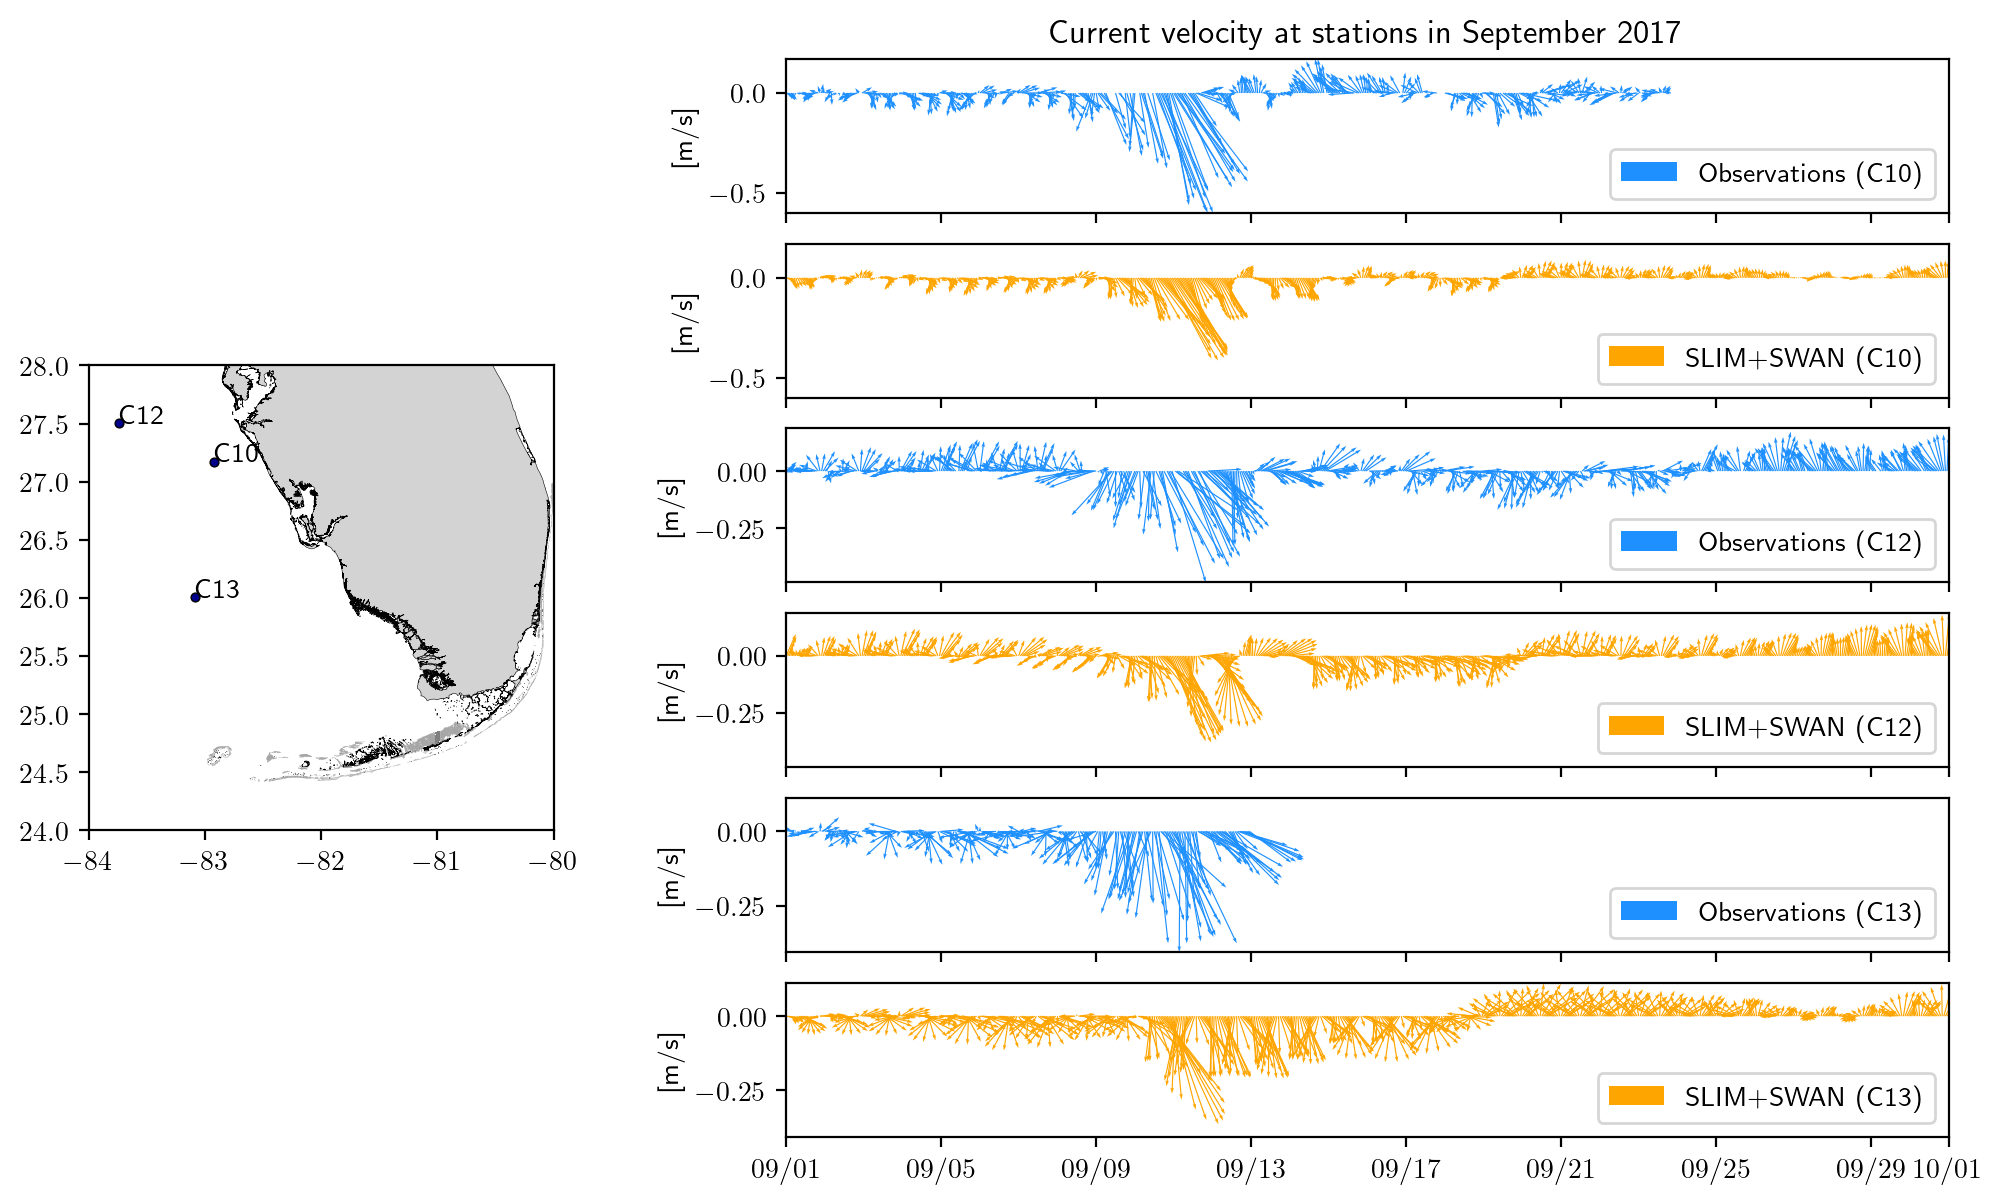
\includegraphics[width=0.9\textwidth]{figures/validation_uv_map.png}
    \caption{Validation of model outputs against ADCP current velocity measurements in September 2017}
    \label{fig:validation}
\end{figure}


% =========================== %
% === DATA AVAILABILITY === %
% =========================== %
\section*{Data availability}
\emphc{The datasets generated during the current study can be accessed \href{https://uclouvain-my.sharepoint.com/:f:/g/personal/thomas_dobbelaere_uclouvain_be/EuRwpuKKnytJvnkfshpBeA8BhwYU19c5sLEe8n3fnPmkjQ?e=pIUMxM}{here}. They will be uploaded on zenodo with a proper doi once the article is ready for publication.}


% =========================== %
% === CODE AVAILABILITY === %
% =========================== %
\section*{Code availability}
The SLIM source code can be found at \href{https://git.immc.ucl.ac.be/slim/slim}{https://git.immc.ucl.ac.be/slim/slim}.


% ================== %
% === REFERENCES === %
% ================== %
\bibliography{sample.bib}


% ======================== %
% === ACKNOWLEDGEMENTS === %
% ======================== %
\section*{Acknowledgements}
Computational resources have been provided by the supercomputing facilities of the \it{Universit\'e catholique de Louvain} (CISM/UCLouvain) and the \it{Consortium des \'Equipements de Calcul Intensif en F\'ed\'eration Wallonie Bruxelles} (CECI) funded by the \it{Fonds de la Recherche Scientifique de Belgique} (F.R.S.-FNRS) under convention 2.5020.11.


% ===================== %
% === CONTRIBUTIONS === %
% ===================== %
\section*{Author contributions statement}
T.D. and E.H. designed the experiment. T.D. and A.D. conducted simulations. T.D., A.S.A. and L.A. designed the models. T.D., A.D. and E.H. wrote the manuscript. All the authors examined the results and reviewed the manuscript.


% =========================== %
% === COMPETING INTERESTS === %
% =========================== %
\section*{Competing interests}
The authors declare no competing interests.

\end{document}
